\documentclass[12pt,a4paper]{article}

\usepackage[utf8]{inputenc}
\usepackage[T1]{fontenc}
\usepackage[portuguese]{babel}
\usepackage{geometry}
\usepackage{amsmath,amssymb,amsthm}
\usepackage{graphicx}
\usepackage{booktabs}
\usepackage{multirow}
\usepackage{float}
\usepackage{xcolor}
\usepackage{listings}
\usepackage{setspace}
\usepackage{hyperref}
\usepackage[ruled,vlined,linesnumbered,portuguese]{algorithm2e}
\usepackage{tikz}
\usetikzlibrary{shapes.geometric, arrows.meta, positioning, calc, decorations.pathreplacing}

\geometry{a4paper, margin=2.4cm}
\setstretch{1.35}

\definecolor{codebg}{rgb}{0.96,0.96,0.94}
\definecolor{codegreen}{rgb}{0.1,0.5,0.1}
\definecolor{codeblue}{rgb}{0.1,0.2,0.65}
\definecolor{codegray}{rgb}{0.45,0.45,0.45}

\lstdefinestyle{cppstyle}{
    backgroundcolor=\color{codebg},
    commentstyle=\color{codegreen}\itshape,
    keywordstyle=\color{codeblue}\bfseries,
    numberstyle=\tiny\color{codegray},
    basicstyle=\ttfamily\footnotesize,
    breaklines=true,
    captionpos=b,
    keepspaces=true,
    numbers=left,
    numbersep=6pt,
    showstringspaces=false,
    tabsize=4,
    frame=single,
    rulecolor=\color{black!20}
}
\lstset{style=cppstyle}

\newtheorem{teorema}{Teorema}[section]
\newtheorem{lema}{Lema}[section]
\newtheorem{definicao}{Defini\c{c}\~ao}[section]

\title{\textbf{Casamento de Cadeias em Sequ\^encias Gen\^omicas: Fundamentos Matem\'aticos, Engenharia e An\'alise Assint\'otica dos Algoritmos de Rabin-Karp e Knuth-Morris-Pratt}}

\author{
    Arthur de Oliveira Mendon\c{c}a \\
    Italo Xavier Fonseca \\
    Thiago Augusto Silva Martins \\
    Thales Guerreiro \\
    Matheus Tavares \\[0.4cm]
    \textit{Departamento de Computa\c{c}\~ao (DECOM-DV) -- CEFET-MG Divin\'opolis} \\
    Disciplina: Algoritmos e Estruturas de Dados II / Projeto e An\'alise de Algoritmos \\
    Professor: Prof. Dr. Michel Pires da Silva
}
\date{Novembro de 2026}

\begin{document}

\maketitle

\begin{abstract}
A localiza\c{c}\~ao exata de subcadeias no interior de grandes volumes textuais constitui um problema cl\'assico da ci\^encia da computa\c{c}\~ao, cuja relev\^ancia pr\'atica se intensificou com o sequenciamento gen\^omico em larga escala. Neste relat\'orio t\'ecnico, investigamos o paradigma de casamento de cadeias (\textit{string matching}) sob a perspectiva te\'orica do Cap\'itulo 32 de Cormen et al. (CLRS) e sob o ponto de vista emp\'irico da bioinform\'atica. Formalizamos a aritm\'etica modular de polin\^omios via Regra de Horner no algoritmo de Rabin-Karp e a teoria de aut\^omatos impl\'icitos baseada na fun\c{c}\~ao de prefixo $\pi$ do algoritmo de Knuth-Morris-Pratt (KMP). Demonstramos analiticamente as cotas assint\'oticas $O$, $\Omega$ e $\Theta$ de tempo e mem\'oria, incluindo a prova amortizada de linearidade $\Theta(n+m)$. Por fim, avaliamos uma implementa\c{c}\~ao de refer\^encia em C++17 aplicada ao genoma completo do v\'irus SARS-CoV-2 (\texttt{NC\_045512.2}) e ao transcrito humano \textit{TP53} (\texttt{NM\_000546.6}), discutindo o papel do casamento exato na etapa de semea\c{c}\~ao (\textit{seeding}) do alinhamento gen\'etico e os gargalos de arquitetura de processadores modernos.
\end{abstract}

\tableofcontents
\newpage

% =============================================================================
% 1. INTRODUCAO
% =============================================================================
\section{Introdu\c{c}\~ao}

A manipula\c{c}\~ao eficiente de cadeias de caracteres sustenta desde ferramentas de busca em editores de c\'odigo e sistemas de detec\c{c}\~ao de intrus\~ao em redes at\'e a montagem e anota\c{c}\~ao de genomas inteiros. Em termos computacionais, o problema consiste em identificar todas as posi\c{c}\~oes onde um padr\~ao $P$ de comprimento $m$ ocorre de maneira cont\'igua dentro de um texto $T$ de comprimento $n$, com $n \ge m$. Quando $n$ se restringe a poucos milhares de caracteres, mesmo uma verifica\c{c}\~ao exaustiva posicional responde em fra\c{c}\~oes de milissegundo. O cen\'ario muda radicalmente na bioinform\'atica moderna. Um \'unico cromossomo humano cont\'em dezenas de milh\~oes de nucleot\'ideos, e um banco de refer\^encia gen\^omica acumula bilh\~oes de bases nitrogenadas representadas sobre o alfabeto quatern\'ario $\Sigma = \{\text{A}, \text{C}, \text{G}, \text{T}\}$.

Historicamente, a abordagem direta para localizar um padr\~ao baseia-se no algoritmo ing\^enuo (ou de for\c{c}a bruta), que desliza o padr\~ao uma posi\c{c}\~ao por vez sobre o texto e compara os caracteres da esquerda para a direita. Essa estrat\'egia padece de uma falha estrutural severa: ela ignora toda a informa\c{c}\~ao obtida nas compara\c{c}\~oes parciais anteriores. Sempre que ocorre uma diverg\^encia no \'indice $j$ do padr\~ao, o ponteiro do texto retrocede para $s+1$ e o processo recome\c{c}a do zero, levando ao custo de pior caso $\Theta((n-m+1)m)$. Em textos de linguagem natural, cujo alfabeto possui dezenas de s\'imbolos, uma falha costuma ocorrer logo na primeira ou segunda letra. No DNA, entretanto, o alfabeto reduzido de apenas quatro letras eleva a probabilidade de coincid\^encia acidental entre duas bases para $25\%$, al\'em de genomas reais conterem extensas regi\~oes repetitivas, como caudas poli-A e microssat\'elites, que for\c{c}am a degrada\c{c}\~ao quadr\'atica da busca ing\^enua.

Paralelamente, na biologia computacional, o alinhamento global ou local de sequ\^encias com muta\c{c}\~oes e lacunas (\textit{gaps}), resolvido pelos algoritmos de programa\c{c}\~ao din\^amica de Needleman-Wunsch e Smith-Waterman, exige tempo $\Theta(nm)$. Executar uma matriz de programa\c{c}\~ao din\^amica contra os $3,2 \times 10^9$ pares de base do genoma humano para cada leitura de sequenciamento \'e computacionalmente proibitivo. Para contornar essa barreira, os alinhadores gen\'eticos reais recorrem aos algoritmos lineares de casamento exato estudados neste trabalho: utiliza-se o \textit{rolling hash} de Rabin-Karp ou aut\^omatos derivados do KMP para localizar rapidamente pequenas sementes exatas (\textit{seeds} ou $k$-mers) em tempo linear, restringindo o alinhamento caro por programa\c{c}\~ao din\^amica apenas \`as regi\~oes candidatas.

O objetivo deste trabalho \'e investigar, formalizar matematicamente e validar experimentalmente os algoritmos de Rabin-Karp e Knuth-Morris-Pratt (KMP), contrastando seu desempenho te\'orico e pr\'atico frente \`a busca ing\^enua em sequ\^encias gen\^omicas reais e sint\'eticas. Buscamos demonstrar n\~ao apenas as provas formais de complexidade assint\'otica do Cap\'itulo 32 de Cormen et al. \cite{cormen2022}, mas tamb\'em expor como fatores de baixo n\'ivel de hardware (como o custo em ciclos de clock da divis\~ao inteira na ALU e a localidade espacial na mem\'oria cache L1) impactam o tempo real de execu\c{c}\~ao em C++17.

O restante deste documento est\'a organizado em cinco cap\'itulos adicionais e um ap\^endice. A Se\c{c}\~ao 2 desenvolve a fundamenta\c{c}\~ao matem\'atica, cobrindo a aritm\'etica modular do Rabin-Karp, o Lema da Superposi\c{c}\~ao de Sufixos e a estrutura da fun\c{c}\~ao de prefixo do KMP. A Se\c{c}\~ao 3 apresenta a engenharia dos algoritmos por meio de pseudoc\'odigos no padr\~ao \texttt{algorithm2e} e diagramas visuais passo a passo. A Se\c{c}\~ao 4 conduz a an\'alise assint\'otica rigorosa ($O$, $\Omega$ e $\Theta$) de tempo e mem\'oria. A Se\c{c}\~ao 5 detalha o estudo de caso em bioinform\'atica com sequ\^encias do NCBI (\texttt{NC\_045512.2} e \texttt{NM\_000546.6}), os experimentos de estresse e a an\'alise de gargalos de hardware. A Se\c{c}\~ao 6 sintetiza as conclus\~oes sobre onde o paradigma \'e aplic\'avel e onde ele falha, seguida pelo Ap\^endice contendo o \textit{Cheat Sheet} de consulta r\'apida.

% =============================================================================
% 2. FUNDAMENTACAO TEORICA
% =============================================================================
\section{Fundamenta\c{c}\~ao Te\'orica}

\subsection{Formaliza\c{c}\~ao do Problema e Nota\c{c}\~oes de Cadeias}

Seja $\Sigma$ um alfabeto finito de s\'imbolos. Na an\'alise gen\^omica, adotamos $\Sigma = \{\text{A}, \text{C}, \text{G}, \text{T}\}$, de cardinalidade $d = |\Sigma| = 4$, ou sua representa\c{c}\~ao em bytes ASCII onde $d = 256$. Definimos o texto como um vetor $T[1..n]$ de comprimento $n$ e o padr\~ao buscado como um vetor $P[1..m]$ de comprimento $m$, com $m \le n$ (adotamos nas demonstra\c{c}\~oes te\'oricas a indexa\c{c}\~ao base-1 do livro-texto de Cormen et al. \cite{cormen2022}, explicitando na Se\c{c}\~ao 5 a transi\c{c}\~ao para base-0 na linguagem C++).

\begin{definicao}[Deslocamento V\'alido e Inv\'alido]
Dizemos que o padr\~ao $P$ ocorre com deslocamento (\textit{shift}) $s$ no texto $T$, onde $0 \le s \le n-m$, se e somente se $T[s+1..s+m] = P[1..m]$, isto \'e, $T[s+j] = P[j]$ para todo $j \in \{1, 2, \dots, m\}$. Se essa igualdade se verifica, $s$ \'e chamado de \textbf{deslocamento v\'alido}; caso contr\'ario, $s$ \'e um \textbf{deslocamento inv\'alido}.
\end{definicao}

Denotamos por $\Sigma^*$ o conjunto de todas as cadeias finitas formadas por caracteres de $\Sigma$, incluindo a cadeia vazia $\varepsilon$ de comprimento zero. Dados $w, x \in \Sigma^*$, escrevemos $w \sqsubset x$ para indicar que $w$ \'e um \textbf{prefixo} de $x$ (existe $y \in \Sigma^*$ tal que $x = wy$) e escrevemos $w \sqsupset x$ para indicar que $w$ \'e um \textbf{sufixo} de $x$ (existe $y \in \Sigma^*$ tal que $x = yw$). Definimos ainda $P_q = P[1..q]$ como o prefixo de $P$ contendo seus primeiros $q$ caracteres, com $P_0 = \varepsilon$.

Um resultado estrutural indispens\'avel para demonstrar a corretude do algoritmo KMP \'e o Lema da Superposi\c{c}\~ao de Sufixos:

\begin{lema}[Lema 32.1 de Cormen et al. -- Superposi\c{c}\~ao de Sufixos]
\label{lema:superposicao}
Sejam $x, y, z \in \Sigma^*$ cadeias tais que $x \sqsupset z$ e $y \sqsupset z$.
\begin{enumerate}
    \item Se $|x| \le |y|$, ent\~ao $x \sqsupset y$.
    \item Se $|x| \ge |y|$, ent\~ao $y \sqsupset x$.
    \item Se $|x| = |y|$, ent\~ao $x = y$.
\end{enumerate}
\end{lema}
\begin{proof}
Se $x \sqsupset z$ e $y \sqsupset z$, ent\~ao existem cadeias $u, v \in \Sigma^*$ tais que $z = ux = vy$. Suponha $|x| \le |y|$. Como $x$ e $y$ coincidem exatamente nos \'ultimos $|x|$ caracteres de $z$, podemos decompor $y$ em $y = wx$, onde $w$ compreende os primeiros $|y| - |x|$ caracteres de $y$. Pela defini\c{c}\~ao de sufixo, conclui-se imediatamente que $x \sqsupset y$. Os casos $|x| \ge |y|$ e $|x| = |y|$ seguem por simetria direta.
\end{proof}

\subsection{Aritm\'etica Modular e \textit{Rolling Hash} no Algoritmo de Rabin-Karp}

Proposto por Karp e Rabin \cite{karp1987}, o algoritmo de Rabin-Karp substitui a compara\c{c}\~ao direta de subcadeias pela compara\c{c}\~ao de assinaturas num\'ericas inteiras. Assumindo que cada caractere $c \in \Sigma$ seja biunivocamente mapeado para um d\'igito em $\{0, 1, \dots, d-1\}$, podemos interpretar qualquer subcadeia de comprimento $m$ como um n\'umero inteiro escrito na base posicional $d$.

Dessa forma, o valor num\'erico $p$ correspondente ao padr\~ao $P[1..m]$ e o valor $t_s$ correspondente \`a subcadeia $T[s+1..s+m]$ na janela de deslocamento $s$ s\~ao definidos pelos polin\^omios:
\begin{equation}
    p = \sum_{i=1}^{m} P[i] \cdot d^{m-i}, \qquad t_s = \sum_{i=1}^{m} T[s+i] \cdot d^{m-i}
\end{equation}

Pela \textbf{Regra de Horner}, ambos $p$ e $t_0$ podem ser avaliados em tempo linear $\Theta(m)$ sem necessidade de exponencia\c{c}\~ao expl\'icita a cada termo:
\begin{equation}
    p = P[m] + d\Big(P[m-1] + d\big(P[m-2] + \dots + d(P[2] + d \cdot P[1])\dots\big)\Big)
\end{equation}

A efici\^encia do algoritmo decorre de podermos calcular $t_{s+1}$ a partir de $t_s$ em tempo constante $\Theta(1)$. Ao deslocar a janela de $s$ para $s+1$, removemos o termo de maior ordem $T[s+1]\cdot d^{m-1}$, multiplicamos o resultado pela base $d$ para elevar o grau dos $m-1$ d\'igitos remanescentes e somamos o novo d\'igito menos significativo $T[s+m+1]$:
\begin{equation}
    t_{s+1} = d \left(t_s - T[s+1]\cdot d^{m-1}\right) + T[s+m+1]
\end{equation}

Quando $m$ \'e moderadamente grande, os valores exatos de $p$ e $t_s$ excedem a capacidade dos registradores nativos da CPU (64 bits). Para manter cada opera\c{c}\~ao aritm\'etica em $\Theta(1)$, todos os c\'alculos s\~ao efetuados no anel de inteiros m\'odulo um n\'umero primo $q$ ($\mathbb{Z}_q$), escolhido de modo que $d \cdot q$ caiba confortavelmente em uma palavra de m\'aquina. Definindo a constante pr\'e-computada $h \equiv d^{m-1} \pmod q$, a recorr\^encia modular do \textit{rolling hash} assume a forma:
\begin{equation}
    \label{eq:rolling_hash}
    t_{s+1} = \Big(d \big(t_s - T[s+1]\cdot h\big) + T[s+m+1]\Big) \bmod q
\end{equation}

A congru\^encia $t_s \equiv p \pmod q$ \'e condi\c{c}\~ao necess\'aria, mas n\~ao suficiente, para que $T[s+1..s+m] = P[1..m]$. Se $t_s \not\equiv p \pmod q$, descartamos o deslocamento $s$ imediatamente em $\Theta(1)$. Se $t_s \equiv p \pmod q$, pode tratar-se de um casamento verdadeiro ou de um \textbf{acerto esp\'urio} (\textit{spurious hit}, uma colis\~ao de hash modular), exigindo a verifica\c{c}\~ao expl\'icita caractere a caractere.

\subsection{A Fun\c{c}\~ao de Prefixo $\pi$ e o Teorema Central do KMP}

O algoritmo desenvolvido por Knuth, Morris e Pratt \cite{knuth1977} elimina completamente a possibilidade de acertos esp\'urios e evita qualquer retrocesso do ponteiro de leitura no texto $T$. Suponha que, no deslocamento atual $s$, os primeiros $q$ caracteres do padr\~ao tenham casado com sucesso, isto \'e, $P[1..q] = T[s+1..s+q]$, mas ocorra uma diverg\^encia no caractere seguinte ($P[q+1] \neq T[s+q+1]$).

Em vez de testar cegamente $s+1$, observamos que os \'ultimos $q$ caracteres lidos do texto s\~ao exatamente conhecidos, pois formam o prefixo $P_q$. Se um novo deslocamento $s' = s + (q - k)$ (com $k < q$) for v\'alido, ent\~ao os primeiros $k$ caracteres do padr\~ao $P_k$ precisam coincidir com os \'ultimos $k$ caracteres de $T[s+1..s+q]$, que s\~ao justamente um sufixo de $P_q$. Isso motiva a defini\c{c}\~ao formal da fun\c{c}\~ao de prefixo:

\begin{definicao}[Fun\c{c}\~ao de Prefixo $\pi$]
Dado um padr\~ao $P[1..m]$, a fun\c{c}\~ao de prefixo para $P$ \'e a aplica\c{c}\~ao $\pi : \{1, 2, \dots, m\} \to \{0, 1, \dots, m-1\}$ tal que $\pi[q]$ \'e o comprimento do maior prefixo de $P$ que \'e um sufixo pr\'oprio de $P_q$:
\begin{equation}
    \pi[q] = \max \{ k : k < q \text{ e } P_k \sqsupset P_q \}
\end{equation}
\end{definicao}

Para construir a tabela $\pi$ eficientemente usando ela pr\'opria, definimos o conjunto de todos os comprimentos de prefixos de $P$ que s\~ao sufixos pr\'oprios de $P_q$ por meio da aplica\c{c}\~ao iterada $\pi^{(u)}[q]$ (onde $\pi^{(1)}[q] = \pi[q]$ e $\pi^{(u)}[q] = \pi[\pi^{(u-1)}[q]]$):
\begin{equation}
    \Pi^*(q) = \big\{ \pi^{(1)}[q], \pi^{(2)}[q], \dots, \pi^{(t)}[q] = 0 \big\}
\end{equation}

\begin{teorema}[Lema da Iteração da Função de Prefixo e Teorema 32.1 de Cormen et al.]
\label{teo:kmp_prefixo}
Para todo $q \in \{1, \dots, m\}$, o conjunto $\Pi^*(q)$ cont\'em exatamente todos os inteiros $k < q$ tais que $P_k \sqsupset P_q$. Ademais, para $q > 1$, se definirmos $E_{q-1} = \{k < q-1 : P_k \sqsupset P_{q-1} \text{ e } P[k+1] = P[q]\}$, ent\~ao:
\begin{equation}
    \pi[q] = \begin{cases}
        0 & \text{se } E_{q-1} = \emptyset, \\
        1 + \max(E_{q-1}) & \text{se } E_{q-1} \neq \emptyset.
    \end{cases}
\end{equation}
\end{teorema}
\begin{proof}
Primeiramente, se $i \in \Pi^*(q)$, ent\~ao pela transitividade da rela\c{c}\~ao $\sqsupset$ tem-se $P_i \sqsupset P_q$ com $i < q$. Reciprocamente, seja $k < q$ qualquer comprimento tal que $P_k \sqsupset P_q$. Pela defini\c{c}\~ao maximal de $\pi[q]$, sabemos que $k \le \pi[q]$ e que ambos $P_k \sqsupset P_q$ e $P_{\pi[q]} \sqsupset P_q$. Aplicando o Lema \ref{lema:superposicao} (Superposi\c{c}\~ao de Sufixos), segue obrigatoriamente que $P_k \sqsupset P_{\pi[q]}$. Se $k = \pi[q]$, ent\~ao $k \in \Pi^*(q)$; se $k < \pi[q]$, repetimos o argumento indutivamente sobre $\pi[\pi[q]]$ at\'e alcan\c{c}ar $k$.

Para a segunda parte, note que $P_r \sqsupset P_q$ para $r > 0$ se e somente se $P[r] = P[q]$ e $P_{r-1} \sqsupset P_{q-1}$. Fazendo $k = r - 1$, vemos que $r - 1 \in E_{q-1}$. Portanto, encontrar o maior $r$ que satisfaz $P_r \sqsupset P_q$ equivale a percorrer os candidatos $k \in \Pi^*(q-1)$ em ordem decrescente ($k = \pi[q-1], \pi[\pi[q-1]], \dots$) at\'e encontrar o primeiro \'indice para o qual $P[k+1] = P[q]$, somando $1$ ao valor encontrado.
\end{proof}

\subsection{Implica\c{c}\~oes em Bioinform\'atica: Do Casamento Exato ao Alinhamento Gen\'etico}

Na pr\'atica bioinform\'atica, duas tarefas distintas costumam ser confundidas: a \textbf{busca exata de motivos/iniciadores} e o \textbf{alinhamento de sequ\^encias hom\'ologas}.
\begin{enumerate}
    \item \textbf{Busca Exata de \textit{Primers}, S\'itios de Restri\c{c}\~ao e \textit{Motifs} Consenso:} No desenho de iniciadores de PCR (\textit{primers} de $18$ a $25$ pb), na busca de s\'itios de clivagem enzim\'atica ou na localiza\c{c}\~ao de caixas promotoras conservadas (como a TATA-box \texttt{TATAAA}), exige-se correspond\^encia exata sobre o cromossomo. O algoritmo KMP resolve essa tarefa em tempo determin\'istico $\Theta(n+m)$, sendo imune \`as regi\~oes de baixa complexidade composicional do DNA.
    \item \textbf{Filtragem e \textit{Seeding} no Alinhamento Gen\'etico (\textit{Seed-and-Extend}):} Durante a evolu\c{c}\~ao biol\'ogica ou o sequenciamento em bancada, ocorrem polimorfismos de nucleot\'ideo \'unico (SNPs), inser\c{c}\~oes e dele\c{c}\~oes (\textit{indels}). Se uma leitura (\textit{read}) de tamanho $m = 120$ pb contiver apenas uma base mutada, tanto KMP quanto Rabin-Karp aplicados \`a leitura inteira retornar\~ao zero casamentos. Contudo, pelo Princ\'ipio da Casa dos Pombos, se uma cadeia de comprimento $m$ possui at\'e $e$ muta\c{c}\~oes pontuais, ao dividirmos ou extrairmos subcadeias cont\'iguas ($k$-mers) de tamanho $k \le \lfloor \frac{m - e}{e + 1} \rfloor$, pelo menos uma dessas sementes permanecer\'a $100\%$ livre de muta\c{c}\~oes. Ferramentas como o BLAST \cite{altschul1990} indexam os $k$-mers da consulta usando \textit{rolling hash} (Rabin-Karp na base $d=4$) para localizar todas as sementes exatas no genoma em $\Theta(n)$ e disparam o alinhamento local de Smith-Waterman restrito \`as diagonais onde as sementes se acumulam.
\end{enumerate}

% =============================================================================
% 3. O PARADIGMA ALGORITMICO (ENGENHARIA DA SOLUCAO)
% =============================================================================
\section{O Paradigma Algor\'itmico (Engenharia da Solu\c{c}\~ao)}

Apresentamos a seguir a especifica\c{c}\~ao formal dos algoritmos utilizando o pacote acad\^emico \texttt{algorithm2e}, acompanhada dos diagramas estruturais de execu\c{c}\~ao passo a passo.

\subsection{Pseudoc\'odigos Formais (\texttt{algorithm2e})}

\begin{algorithm}[H]
\DontPrintSemicolon
\SetAlgoLined
\KwIn{Texto $T[1..n]$ e padr\~ao $P[1..m]$ sobre o alfabeto $\Sigma$.}
\KwOut{Deslocamentos v\'alidos $s$ onde $P$ ocorre em $T$.}
$n \leftarrow T.\text{comprimento}$\;
$m \leftarrow P.\text{comprimento}$\;
\Para{$s \leftarrow 0$ \KwTo $n - m$}{
    $j \leftarrow 1$\;
    \Enqto{$j \le m$ \textbf{e} $T[s + j] == P[j]$}{
        $j \leftarrow j + 1$\;
    }
    \Se{$j > m$}{
        \textbf{imprimir} ``Padr\~ao ocorre com deslocamento v\'alido '' $s$\;
    }
}
\caption{\textsc{Casador-Ingenuo-Cadeias}$(T, P)$}
\label{alg:naive}
\end{algorithm}

\vspace{0.3cm}

\begin{algorithm}[H]
\DontPrintSemicolon
\SetAlgoLined
\KwIn{Texto $T[1..n]$, padr\~ao $P[1..m]$, base $d = |\Sigma|$ e primo $q$.}
\KwOut{Deslocamentos v\'alidos $s$ onde $P$ ocorre em $T$.}
$n \leftarrow T.\text{comprimento}$\;
$m \leftarrow P.\text{comprimento}$\;
$h \leftarrow d^{m-1} \bmod q$\;
$p \leftarrow 0$\;
$t_0 \leftarrow 0$\;
\tcp{Pr\'e-processamento via Regra de Horner em $\Theta(m)$}
\Para{$i \leftarrow 1$ \KwTo $m$}{
    $p \leftarrow (d \cdot p + P[i]) \bmod q$\;
    $t_0 \leftarrow (d \cdot t_0 + T[i]) \bmod q$\;
}
\tcp{Etapa de casamento por janela deslizante (Rolling Hash)}
\Para{$s \leftarrow 0$ \KwTo $n - m$}{
    \Se{$p == t_s$}{
        \Se{$P[1..m] == T[s+1..s+m]$}{
            \textbf{imprimir} ``Padr\~ao ocorre com deslocamento v\'alido '' $s$\;
        }
    }
    \Se{$s < n - m$}{
        $t_{s+1} \leftarrow \big(d \cdot (t_s - T[s+1]\cdot h) + T[s+m+1]\big) \bmod q$\;
        \Se{$t_{s+1} < 0$}{
            $t_{s+1} \leftarrow t_{s+1} + q$\;
        }
    }
}
\caption{\textsc{Casador-Rabin-Karp}$(T, P, d, q)$}
\label{alg:rk}
\end{algorithm}

\newpage

\begin{algorithm}[H]
\DontPrintSemicolon
\SetAlgoLined
\KwIn{Padr\~ao $P[1..m]$.}
\KwOut{Vetor da fun\c{c}\~ao de prefixo $\pi[1..m]$.}
$m \leftarrow P.\text{comprimento}$\;
Seja $\pi[1..m]$ um novo vetor\;
$\pi[1] \leftarrow 0$\;
$k \leftarrow 0$\;
\Para{$q \leftarrow 2$ \KwTo $m$}{
    \Enqto{$k > 0$ \textbf{e} $P[k + 1] \neq P[q]$}{
        $k \leftarrow \pi[k]$\;
    }
    \Se{$P[k + 1] == P[q]$}{
        $k \leftarrow k + 1$\;
    }
    $\pi[q] \leftarrow k$\;
}
\Retorna{$\pi$}\;
\caption{\textsc{Calcular-Funcao-Prefixo}$(P)$}
\label{alg:pi}
\end{algorithm}

\vspace{0.3cm}

\begin{algorithm}[H]
\DontPrintSemicolon
\SetAlgoLined
\KwIn{Texto $T[1..n]$ e padr\~ao $P[1..m]$.}
\KwOut{Deslocamentos v\'alidos $s$ onde $P$ ocorre em $T$.}
$n \leftarrow T.\text{comprimento}$\;
$m \leftarrow P.\text{comprimento}$\;
$\pi \leftarrow \textsc{Calcular-Funcao-Prefixo}(P)$\;
$q \leftarrow 0$ \tcp*{N\'umero de caracteres casados no estado atual}
\Para{$i \leftarrow 1$ \KwTo $n$}{
    \Enqto{$q > 0$ \textbf{e} $P[q + 1] \neq T[i]$}{
        $q \leftarrow \pi[q]$\;
    }
    \Se{$P[q + 1] == T[i]$}{
        $q \leftarrow q + 1$\;
    }
    \Se{$q == m$}{
        \textbf{imprimir} ``Padr\~ao ocorre com deslocamento '' $(i - m)$\;
        $q \leftarrow \pi[q]$\;
    }
}
\caption{\textsc{Casador-KMP}$(T, P)$}
\label{alg:kmp}
\end{algorithm}

\subsection{Diagramas Visuais Passo a Passo}

A Figura \ref{fig:tikz_rk} ilustra o mecanismo alg\'ebrico de atualiza\c{c}\~ao em $\Theta(1)$ da janela deslizante no algoritmo de Rabin-Karp sobre uma fita de DNA mapeada em base $d=4$ ($\text{A}=0, \text{C}=1, \text{G}=2, \text{T}=3$).

\begin{figure}[H]
\centering
\begin{tikzpicture}[scale=0.92, every node/.style={transform shape}]
    % Passo s
    \node[anchor=west, font=\bfseries\small] at (0, 2.5) {Janela $s$: $T[s+1..s+4] = \texttt{T A T A}$};
    \draw[fill=red!18, draw=red!70, thick] (0, 1.4) rectangle (1.1, 2.2) node[pos=.5, font=\ttfamily\bfseries] {T(3)};
    \draw[fill=blue!10, draw=blue!60, thick] (1.1, 1.4) rectangle (2.2, 2.2) node[pos=.5, font=\ttfamily\bfseries] {A(0)};
    \draw[fill=blue!10, draw=blue!60, thick] (2.2, 1.4) rectangle (3.3, 2.2) node[pos=.5, font=\ttfamily\bfseries] {T(3)};
    \draw[fill=blue!10, draw=blue!60, thick] (3.3, 1.4) rectangle (4.4, 2.2) node[pos=.5, font=\ttfamily\bfseries] {A(0)};
    \draw[fill=gray!10, draw=gray!60] (4.4, 1.4) rectangle (5.5, 2.2) node[pos=.5, font=\ttfamily] {A(0)};
    \draw[fill=gray!10, draw=gray!60] (5.5, 1.4) rectangle (6.6, 2.2) node[pos=.5, font=\ttfamily] {G(2)};

    % Passo s+1
    \node[anchor=west, font=\bfseries\small] at (0, 0.5) {Janela $s+1$: $T[s+2..s+5] = \texttt{A T A A}$};
    \draw[fill=gray!10, draw=gray!60] (0, -0.6) rectangle (1.1, 0.2) node[pos=.5, font=\ttfamily] {T(3)};
    \draw[fill=blue!10, draw=blue!60, thick] (1.1, -0.6) rectangle (2.2, 0.2) node[pos=.5, font=\ttfamily\bfseries] {A(0)};
    \draw[fill=blue!10, draw=blue!60, thick] (2.2, -0.6) rectangle (3.3, 0.2) node[pos=.5, font=\ttfamily\bfseries] {T(3)};
    \draw[fill=blue!10, draw=blue!60, thick] (3.3, -0.6) rectangle (4.4, 0.2) node[pos=.5, font=\ttfamily\bfseries] {A(0)};
    \draw[fill=green!20, draw=green!60!black, thick] (4.4, -0.6) rectangle (5.5, 0.2) node[pos=.5, font=\ttfamily\bfseries] {A(0)};
    \draw[fill=gray!10, draw=gray!60] (5.5, -0.6) rectangle (6.6, 0.2) node[pos=.5, font=\ttfamily] {G(2)};

    % Caixa de equacao a direita
    \node[draw=black!60, rounded corners, fill=yellow!8, inner sep=8pt, text width=7.6cm, anchor=west, font=\footnotesize] at (7.3, 0.8) {
        \textbf{Transi\c{c}\~ao em Tempo Constante $\Theta(1)$:}\\[4pt]
        1. \textcolor{red!80!black}{\textbf{Remove}} a base que sai pela esquerda:\\
        $\quad t'_s = t_s - T[s+1]\cdot d^{m-1}$\\[3pt]
        2. \textcolor{blue!80!black}{\textbf{Desloca}} as $m-1$ bases restantes ($\times d$):\\
        $\quad t''_s = d \cdot t'_s$\\[3pt]
        3. \textcolor{green!50!black}{\textbf{Soma}} a nova base que entra pela direita:\\
        $\quad t_{s+1} = (t''_s + T[s+m+1]) \bmod q$
    };
\end{tikzpicture}
\caption{Diagrama de atualiza\c{c}\~ao incremental do \textit{Rolling Hash} no algoritmo de Rabin-Karp.}
\label{fig:tikz_rk}
\end{figure}

A Figura \ref{fig:tikz_kmp} demonstra o comportamento do KMP e da tabela $\pi$ diante de uma falha ap\'os casar $q = 5$ bases do padr\~ao $P = \texttt{ACAGAC}$. Observando o prefixo casado $P_5 = \texttt{ACAGA}$, verifica-se que o maior prefixo pr\'oprio de $P$ que tamb\'em \'e sufixo de $P_5$ \'e $P_1 = \texttt{A}$ ($\pi[5] = 1$). Assim, o padr\~ao desliza diretamente $q - \pi[q] = 5 - 1 = 4$ posi\c{c}\~oes sem retroceder o \'indice de leitura do texto.

\begin{figure}[H]
\centering
\begin{tikzpicture}[scale=0.9, every node/.style={transform shape}]
    % Tabela pi no topo
    \node[anchor=west, font=\bfseries\small] at (0, 3.6) {Tabela de Prefixo $\pi$ para $P = \texttt{A C A G A C}$:};
    \foreach \idx/\ch/\pval in {1/A/0, 2/C/0, 3/A/1, 4/G/0, 5/A/1, 6/C/2} {
        \draw[fill=gray!15] (\idx*1.0, 2.8) rectangle (\idx*1.0+1.0, 3.3) node[pos=.5, font=\scriptsize] {$q=\idx$};
        \draw[fill=white] (\idx*1.0, 2.2) rectangle (\idx*1.0+1.0, 2.8) node[pos=.5, font=\ttfamily\bfseries] {\ch};
        \draw[fill=blue!12] (\idx*1.0, 1.6) rectangle (\idx*1.0+1.0, 2.2) node[pos=.5, font=\bfseries] {$\pval$};
    }
    \node[anchor=east, font=\scriptsize\bfseries] at (0.95, 3.05) {\'Indice:};
    \node[anchor=east, font=\scriptsize\bfseries] at (0.95, 2.5) {$P[q]$:};
    \node[anchor=east, font=\scriptsize\bfseries] at (0.95, 1.9) {$\pi[q]$:};

    % Estado antes da falha (s=0, q=5 casados, falha no 6)
    \node[anchor=west, font=\footnotesize\bfseries] at (8.2, 3.1) {Falha em $q=5$ ($P[6]=\texttt{C} \neq T[6]=\texttt{G}$):};
    \foreach \i/\c in {1/A, 2/C, 3/A, 4/G, 5/A, 6/G, 7/A, 8/C} {
        \draw[fill=gray!10] (7.4+\i*0.8, 2.2) rectangle (8.2+\i*0.8, 2.8) node[pos=.5, font=\ttfamily\small] {\c};
    }
    \foreach \i/\c in {1/A, 2/C, 3/A, 4/G, 5/A} {
        \draw[fill=green!18, draw=green!60!black, thick] (7.4+\i*0.8, 1.4) rectangle (8.2+\i*0.8, 2.0) node[pos=.5, font=\ttfamily\small\bfseries] {\c};
    }
    \draw[fill=red!22, draw=red!70!black, thick] (7.4+6*0.8, 1.4) rectangle (8.2+6*0.8, 2.0) node[pos=.5, font=\ttfamily\small\bfseries] {C};

    % Seta de deslocamento inteligente s' = s + (q - pi[q]) = 0 + (5 - 1) = 4
    \draw[-{Stealth[length=3mm]}, ultra thick, blue!70!black] (8.6, 1.2) -- (11.8, 0.5) node[midway, below left, font=\scriptsize\bfseries] {Salto $q \leftarrow \pi[5] = 1$ ($\Delta s = 4$)};

    \foreach \i/\c in {1/A, 2/C, 3/A, 4/G, 5/A, 6/C} {
        \pgfmathsetmacro{\xcoord}{7.4 + (\i+4)*0.8}
        \ifnum\i=1
            \draw[fill=blue!20, draw=blue!70!black, thick] (\xcoord, -0.2) rectangle (\xcoord+0.8, 0.4) node[pos=.5, font=\ttfamily\small\bfseries] {\c};
        \else
            \draw[fill=white, draw=black!50] (\xcoord, -0.2) rectangle (\xcoord+0.8, 0.4) node[pos=.5, font=\ttfamily\small] {\c};
        \fi
    }
\end{tikzpicture}
\caption{Representa\c{c}\~ao da tabela $\pi$ e do salto determin\'istico do KMP sem retrocesso no texto $T$.}
\label{fig:tikz_kmp}
\end{figure}

Por fim, a Figura \ref{fig:tikz_seeding} apresenta o fluxograma da integra\c{c}\~ao dos algoritmos de casamento exato dentro de uma pipeline de alinhamento gen\'etico (\textit{Seed-and-Extend}).

\begin{figure}[H]
\centering
\begin{tikzpicture}[
    node distance=1.2cm and 1.4cm,
    box/.style={rectangle, rounded corners, draw=black!75, thick, fill=blue!8, text width=3.4cm, align=center, minimum height=1.1cm, font=\footnotesize\bfseries},
    decision/.style={diamond, aspect=2.1, draw=black!75, thick, fill=orange!12, text width=2.5cm, align=center, font=\footnotesize\bfseries},
    arrow/.style={-{Stealth[length=2.8mm]}, thick}
]
    \node[box] (read) {Leitura de DNA (\textit{Read}) $m$ pb + Genoma $T$};
    \node[box, right=of read] (kmer) {Extração de $k$-mers e \textit{Rolling Hash} (Rabin-Karp)};
    \node[decision, right=of kmer] (hit) {Hash $t_s \equiv p$ e Semente Exata?};
    \node[box, below=1.0cm of hit, fill=green!12] (dp) {Alinhamento Local Restrito (Smith-Waterman na Diagonal)};
    \node[box, left=of dp, fill=gray!15] (skip) {Avança Janela em $\Theta(1)$ (Descarta Região)};

    \draw[arrow] (read) -- (kmer);
    \draw[arrow] (kmer) -- (hit);
    \draw[arrow] (hit) -- node[right, font=\scriptsize\bfseries] {Sim (\^Ancora)} (dp);
    \draw[arrow] (hit) -- node[above left, font=\scriptsize\bfseries] {N\~ao} (skip);
    \draw[arrow] (skip) -- (kmer);
\end{tikzpicture}
\caption{Fluxograma da etapa de \textit{Seeding} via casamento exato acoplada ao alinhamento gen\'etico.}
\label{fig:tikz_seeding}
\end{figure}

% =============================================================================
% 4. ANALISE ASSINTOTICA RIGOROSA (CUSTOS)
% =============================================================================
\section{An\'alise Assint\'otica Rigorosa (Custos)}

Realizamos nesta se\c{c}\~ao o estudo formal das cotas superiores ($O$), inferiores ($\Omega$) e restritas ($\Theta$) de tempo de processamento e consumo de mem\'oria para os tr\^es algoritmos.

\subsection{Complexidade da Busca Ing\^enua}
O Algoritmo \ref{alg:naive} n\~ao possui etapa de pr\'e-processamento ($T_{\text{pre}} = \Theta(1)$) e utiliza apenas vari\'aveis escalares de controle ($S(n,m) = \Theta(1)$).
\begin{itemize}
    \item \textbf{Melhor Caso -- $\Omega(n)$:} Ocorre quando o primeiro caractere do padr\~ao nunca coincide com o texto ($T[s+1] \neq P[1]$ para todo $s$). O la\c{c}o interno executa exatamente $1$ compara\c{c}\~ao para cada um dos $n - m + 1$ deslocamentos, totalizando $n - m + 1 = \Omega(n)$ opera\c{c}\~oes.
    \item \textbf{Pior Caso -- $\Theta((n - m + 1)m)$:} Ocorre em cadeias peri\'odicas ou constantes, como $T = \texttt{A}^n$ e $P = \texttt{A}^{m-1}\texttt{C}$. Para cada um dos $n - m + 1$ deslocamentos, o la\c{c}o interno executa exatamente $m$ compara\c{c}\~oes antes de falhar no \'ultimo caractere. O n\'umero exato de compara\c{c}\~oes \'e $(n - m + 1)m = \Theta((n - m + 1)m)$, que atinge $\Theta(n^2)$ quando $m = \lfloor n/2 \rfloor$.
    \item \textbf{Caso M\'edio sobre o Alfabeto do DNA ($|\Sigma| = 4$) -- $\Theta(n)$:} Assumindo bases independentes e uniformemente distribu\'idas com probabilidade $p_c = 1/|\Sigma| = 1/4$, o n\'umero esperado de compara\c{c}\~oes em um deslocamento arbitr\'ario \'e limitado pela s\'erie geom\'etrica:
    \begin{equation}
        \mathbb{E}[C_s] = \sum_{j=1}^{m} \left(\frac{1}{|\Sigma|}\right)^{j-1} < \frac{1}{1 - 1/|\Sigma|} = \frac{4}{3} \approx 1,333\text{ compara\c{c}\~oes por posi\c{c}\~ao.}
    \end{equation}
    Pela linearidade da esperan\c{c}a, o total esperado de compara\c{c}\~oes sobre o texto \'e $\frac{4}{3}(n - m + 1) = \Theta(n)$.
\end{itemize}

\subsection{Complexidade do Algoritmo de Rabin-Karp}
\begin{itemize}
    \item \textbf{Pr\'e-processamento -- $\Theta(m)$:} O la\c{c}o das linhas 6 a 9 do Algoritmo \ref{alg:rk} aplica a Regra de Horner exatamente $m$ vezes, executando $\Theta(m)$ opera\c{c}\~oes aritm\'eticas modulares.
    \item \textbf{Melhor Caso de Busca -- $\Omega(n - m + 1)$:} Se o padr\~ao n\~ao ocorre no texto e n\~ao h\'a colis\~oes esp\'urias, cada janela realiza apenas a compara\c{c}\~ao inteira $p == t_s$ e a atualiza\c{c}\~ao da Equa\c{c}\~ao (\ref{eq:rolling_hash}) em $\Theta(1)$, resultando em $\Theta(n - m + 1)$.
    \item \textbf{Pior Caso de Busca -- $\Theta((n - m + 1)m)$:} Se todos os deslocamentos tiverem $t_s \equiv p \pmod q$ (por exemplo, $T = \texttt{A}^n$ e $P = \texttt{A}^m$, ou escolha patol\'ogica de $q$), a verifica\c{c}\~ao caractere a caractere de custo $\Theta(m)$ \'e acionada em todas as $n - m + 1$ janelas.
    \item \textbf{Caso M\'edio de Busca -- $O(n + m)$:} Supondo que o m\'odulo $q$ atue como uma fun\c{c}\~ao de dispers\~ao uniforme sobre $\mathbb{Z}_q$, a probabilidade de dois hashes distintos colidirem modulo $q$ \'e $1/q$. Com $\nu$ ocorr\^encias v\'alidas no texto, o n\'umero esperado de colis\~oes esp\'urias \'e $O((n - m + 1)/q)$. Cada verifica\c{c}\~ao custa $O(m)$, fornecendo o tempo esperado total:
    \begin{equation}
        \mathbb{E}[T_{\text{busca}}] = O(n) + O\left(m \left(\nu + \frac{n}{q}\right)\right)
    \end{equation}
    Escolhendo um primo $q \ge m$ (na pr\'atica $q = 10^9 + 7 \gg n$), o termo $mn/q$ torna-se inferior a $O(n)$, garantindo tempo esperado $\Theta(n + m)$ quando $\nu = O(1)$.
    \item \textbf{Complexidade de Espa\c{c}o -- $\Theta(1)$:} O algoritmo armazena apenas os inteiros escalares $p, t_s, h, d, q$, consumindo mem\'oria auxiliar constante.
\end{itemize}

\subsection{Complexidade Amortizada Rigorosa do Algoritmo KMP}

A grande virtude te\'orica do KMP reside no fato de que seu melhor caso, caso m\'edio e pior caso coincidem assintoticamente em $\Theta(n + m)$.

\begin{teorema}[Custo Linear $\Theta(m)$ de \textsc{Calcular-Funcao-Prefixo}]
O Algoritmo \ref{alg:pi} calcula o vetor $\pi[1..m]$ em tempo estritamente $\Theta(m)$ no pior caso.
\end{teorema}
\begin{proof}
Utilizamos o \textbf{m\'etodo da fun\c{c}\~ao potencial} (ou m\'etodo agregado) sobre a vari\'avel inteira $k$:
\begin{enumerate}
    \item Inicialmente, na linha 4, temos $k = 0$, e o invariante $0 \le k < q$ mant\'em-se em todas as itera\c{c}\~oes, garantindo que $k \ge 0$ nunca assume valores negativos.
    \item O \'unico ponto do algoritmo onde $k$ aumenta \'e na linha 10 ($k \leftarrow k + 1$), que \'e executada no m\'aximo uma vez por itera\c{c}\~ao do la\c{c}o \textbf{para} externo ($q = 2, \dots, m$). Logo, ao longo de toda a execu\c{c}\~ao do procedimento, $k$ sofre no m\'aximo $m - 1$ incrementos unit\'arios.
    \item No interior do la\c{c}o \textbf{enquanto} (linha 7), a atribui\c{c}\~ao $k \leftarrow \pi[k]$ substitui $k$ por um valor estritamente menor, pois pela defini\c{c}\~ao da fun\c{c}\~ao de prefixo temos $\pi[k] < k$, implicando que cada itera\c{c}\~ao do la\c{c}o \textbf{enquanto} reduz $k$ em pelo menos $1$ unidade ($\Delta k \le -1$).
    \item Como $k$ parte de $0$, nunca fica negativo e sobe no m\'aximo $m - 1$ unidades no total, o la\c{c}o \textbf{enquanto} n\~ao pode executar mais do que $m - 1$ vezes somando todas as $m - 1$ itera\c{c}\~oes do la\c{c}o \textbf{para}.
\end{enumerate}
Consequentemente, o custo total de todas as compara\c{c}\~oes e atribui\c{c}\~oes \'e limitado superiormente por $2(m - 1)$ opera\c{c}\~oes e inferiormente pelas $m - 1$ itera\c{c}\~oes do la\c{c}o externo, provando que $T_{\text{pre}}(m) = \Theta(m)$.
\end{proof}

\begin{teorema}[Custo Linear $\Theta(n)$ de \textsc{Casador-KMP}]
A etapa de busca do Algoritmo \ref{alg:kmp} executa em tempo estritamente $\Theta(n)$ no pior caso, realizando no m\'aximo $2n$ compara\c{c}\~oes de caracteres.
\end{teorema}
\begin{proof}
Aplicamos o mesmo argumento potencial sobre o estado $q$ (n\'umero de caracteres casados):
\begin{enumerate}
    \item O estado $q$ inicia em $0$ e satisfaz $0 \le q \le m$ durante todo o la\c{c}o principal ($i = 1, \dots, n$).
    \item Em cada uma das $n$ itera\c{c}\~oes do la\c{c}o \textbf{para}, a condicional da linha 9 incrementa $q$ em no m\'aximo $1$ unidade ($q \leftarrow q + 1$). Portanto, a soma total de aumentos de $q$ em toda a busca \'e no m\'aximo $n$.
    \item Cada itera\c{c}\~ao do la\c{c}o \textbf{enquanto} (linha 7, $q \leftarrow \pi[q]$) e cada redefini\c{c}\~ao ap\'os casamento completo (linha 13) reduz $q$ em pelo menos $1$ unidade, visto que $\pi[q] \le q - 1$.
    \item Como $q \ge 0$ sempre se verifica, o n\'umero total acumulado de execu\c{c}\~oes do corpo do la\c{c}o \textbf{enquanto} ao longo de todas as $n$ posi\c{c}\~oes do texto \'e no m\'aximo $n$.
\end{enumerate}
Somando no m\'aximo $n$ compara\c{c}\~oes bem-sucedidas (ou falhas em $q=0$) na linha 8 com no m\'aximo $n$ compara\c{c}\~oes que falham no la\c{c}o \textbf{enquanto}, o algoritmo realiza no m\'aximo $2n$ compara\c{c}\~oes de caracteres e no m\'inimo $n$ compara\c{c}\~oes, resultando em $T_{\text{busca}}(n) = \Theta(n)$ e custo global $\Theta(n + m)$. O consumo de mem\'oria auxiliar \'e $\Theta(m)$ devido \`a aloca\c{c}\~ao do vetor $\pi[1..m]$.
\end{proof}

% =============================================================================
% 5. ESTUDO DE CASO E IMPLEMENTACAO PRATICA
% =============================================================================
\section{Estudo de Caso e Implementa\c{c}\~ao Pr\'atica}

\subsection{Arquitetura do Reposit\'orio e Ambiente de Testes}

Todo o c\'odigo-fonte em C++17, os conjuntos de dados gen\^omicos em formato FASTA e os scripts de automa\c{c}\~ao de gr\'aficos encontram-se dispon\'iveis publicamente no reposit\'orio oficial da equipe no GitHub:
\begin{center}
    \url{https://github.com/ImArthz/Aeds2_casamento_de_cadeias.git}
\end{center}

{\sloppy A solu\c{c}\~ao foi estruturada nos m\'odulos \texttt{include/casamento\_cadeias.hpp} e \texttt{src/casamento\_cadeias.cpp} (contendo as implementa\c{c}\~oes instrumentadas de busca ing\^enua, Rabin-Karp, KMP e o motor de \textit{seeding} de $k$-mers), \texttt{src/fasta\_io.cpp} (leitor de arquivos FASTA e gerador de sequ\^encias sint\'eticas de DNA) e \texttt{src/main.cpp}. O c\'odigo foi compilado com otimiza\c{c}\~ao m\'axima (\texttt{-std=c++17 -O3}) para avalia\c{c}\~ao fiel ao n\'ivel de m\'aquina.\par}

Para validar o comportamento em dados biol\'ogicos reais, coletamos do banco de dados \textbf{NCBI RefSeq} duas sequ\^encias de refer\^encia:
\begin{enumerate}
    \item \textbf{Genoma completo do SARS-CoV-2 (\texttt{NC\_045512.2}):} Isolado Wuhan-Hu-1, possuindo $n = 29.903$ pares de base (pb), encerrado por uma cauda poli-A real de $33$ adeninas consecutivas na extremidade $3'$.
    \item \textbf{Transcrito humano \textit{TP53} (\texttt{NM\_000546.6}):} RNA mensageiro da prote\'ina supressora tumoral p53 humana, com $n = 2.512$ pb.
\end{enumerate}

\subsection{Experimento 1: Busca de Padr\~oes Biol\'ogicos no Genoma do SARS-CoV-2}

Executamos os algoritmos sobre os $29.903$ pb do SARS-CoV-2 buscando quatro alvos biol\'ogicos distintos: (i) o motivo promotor \textbf{TATA-box} (\texttt{TATAAA}, $m=6$, consenso JASPAR \texttt{MA0108.2}); (ii) o iniciador diagn\'ostico de RT-PCR da OMS \textbf{RdRp\_SARSr-F2} (\texttt{GTGAAATGGTCATGTGTGGCGG}, $m=22$); (iii) o \textbf{s\'itio de clivagem da furina} na glicoprote\'ina Spike (\texttt{CCTCGGCGGGCACGTAGT}, $m=18$); e (iv) um segmento de \textbf{cauda poli-A} (\texttt{A}$^{25}$, $m=25$). Os resultados medidos encontram-se na Tabela \ref{tab:genoma_real} e na Figura \ref{fig:genoma_sars}.

\begin{table}[H]
\centering
\footnotesize
\resizebox{\textwidth}{!}{\begin{tabular}{@{}llrrrr@{}}
\toprule
\textbf{Padr\~ao Biol\'ogico} & \textbf{Algoritmo} & \textbf{Hits} & \textbf{Compara\c{c}\~oes} & \textbf{Colis\~oes} & \textbf{Tempo Total (ms)} \\ \midrule
\multirow{4}{*}{Motif TATA-box ($m=6$)} 
 & Ing\^enuo & 20 & 42.688 & 0 & 0,1137 \\
 & Rabin-Karp ($q=10^9+7$) & 20 & 120 & 0 & 0,1226 \\
 & Rabin-Karp ($q=101$) & 20 & 412 & 197 & 0,1254 \\
 & KMP & 20 & 42.503 & 0 & 0,1336 \\ \midrule
\multirow{4}{*}{Primer OMS RdRp-F2 ($m=22$)} 
 & Ing\^enuo & 1 & 38.495 & 0 & 0,0818 \\
 & Rabin-Karp ($q=10^9+7$) & 1 & 22 & 0 & 0,1212 \\
 & Rabin-Karp ($q=101$) & 1 & 386 & 288 & 0,1247 \\
 & KMP & 1 & 38.403 & 0 & 0,1084 \\ \midrule
\multirow{4}{*}{S\'itio Furina Spike ($m=18$)} 
 & Ing\^enuo & 1 & 36.685 & 0 & 0,0693 \\
 & Rabin-Karp ($q=10^9+7$) & 1 & 18 & 0 & 0,1245 \\
 & Rabin-Karp ($q=101$) & 1 & 366 & 285 & 0,1244 \\
 & KMP & 1 & 36.371 & 0 & 0,0923 \\ \midrule
\multirow{4}{*}{Cauda Poli-A ($m=25$)} 
 & Ing\^enuo & 9 & 43.065 & 0 & 0,0906 \\
 & Rabin-Karp ($q=10^9+7$) & 9 & 225 & 0 & 0,1217 \\
 & Rabin-Karp ($q=101$) & 9 & 660 & 304 & 0,1255 \\
 & KMP & 9 & 41.751 & 0 & 0,1562 \\ \bottomrule
\end{tabular}}
\caption{M\'etricas emp\'iricas de busca exata no genoma real do SARS-CoV-2 (\texttt{NC\_045512.2}, $29.903$ pb).}
\label{tab:genoma_real}
\end{table}

\begin{figure}[H]
    \centering
    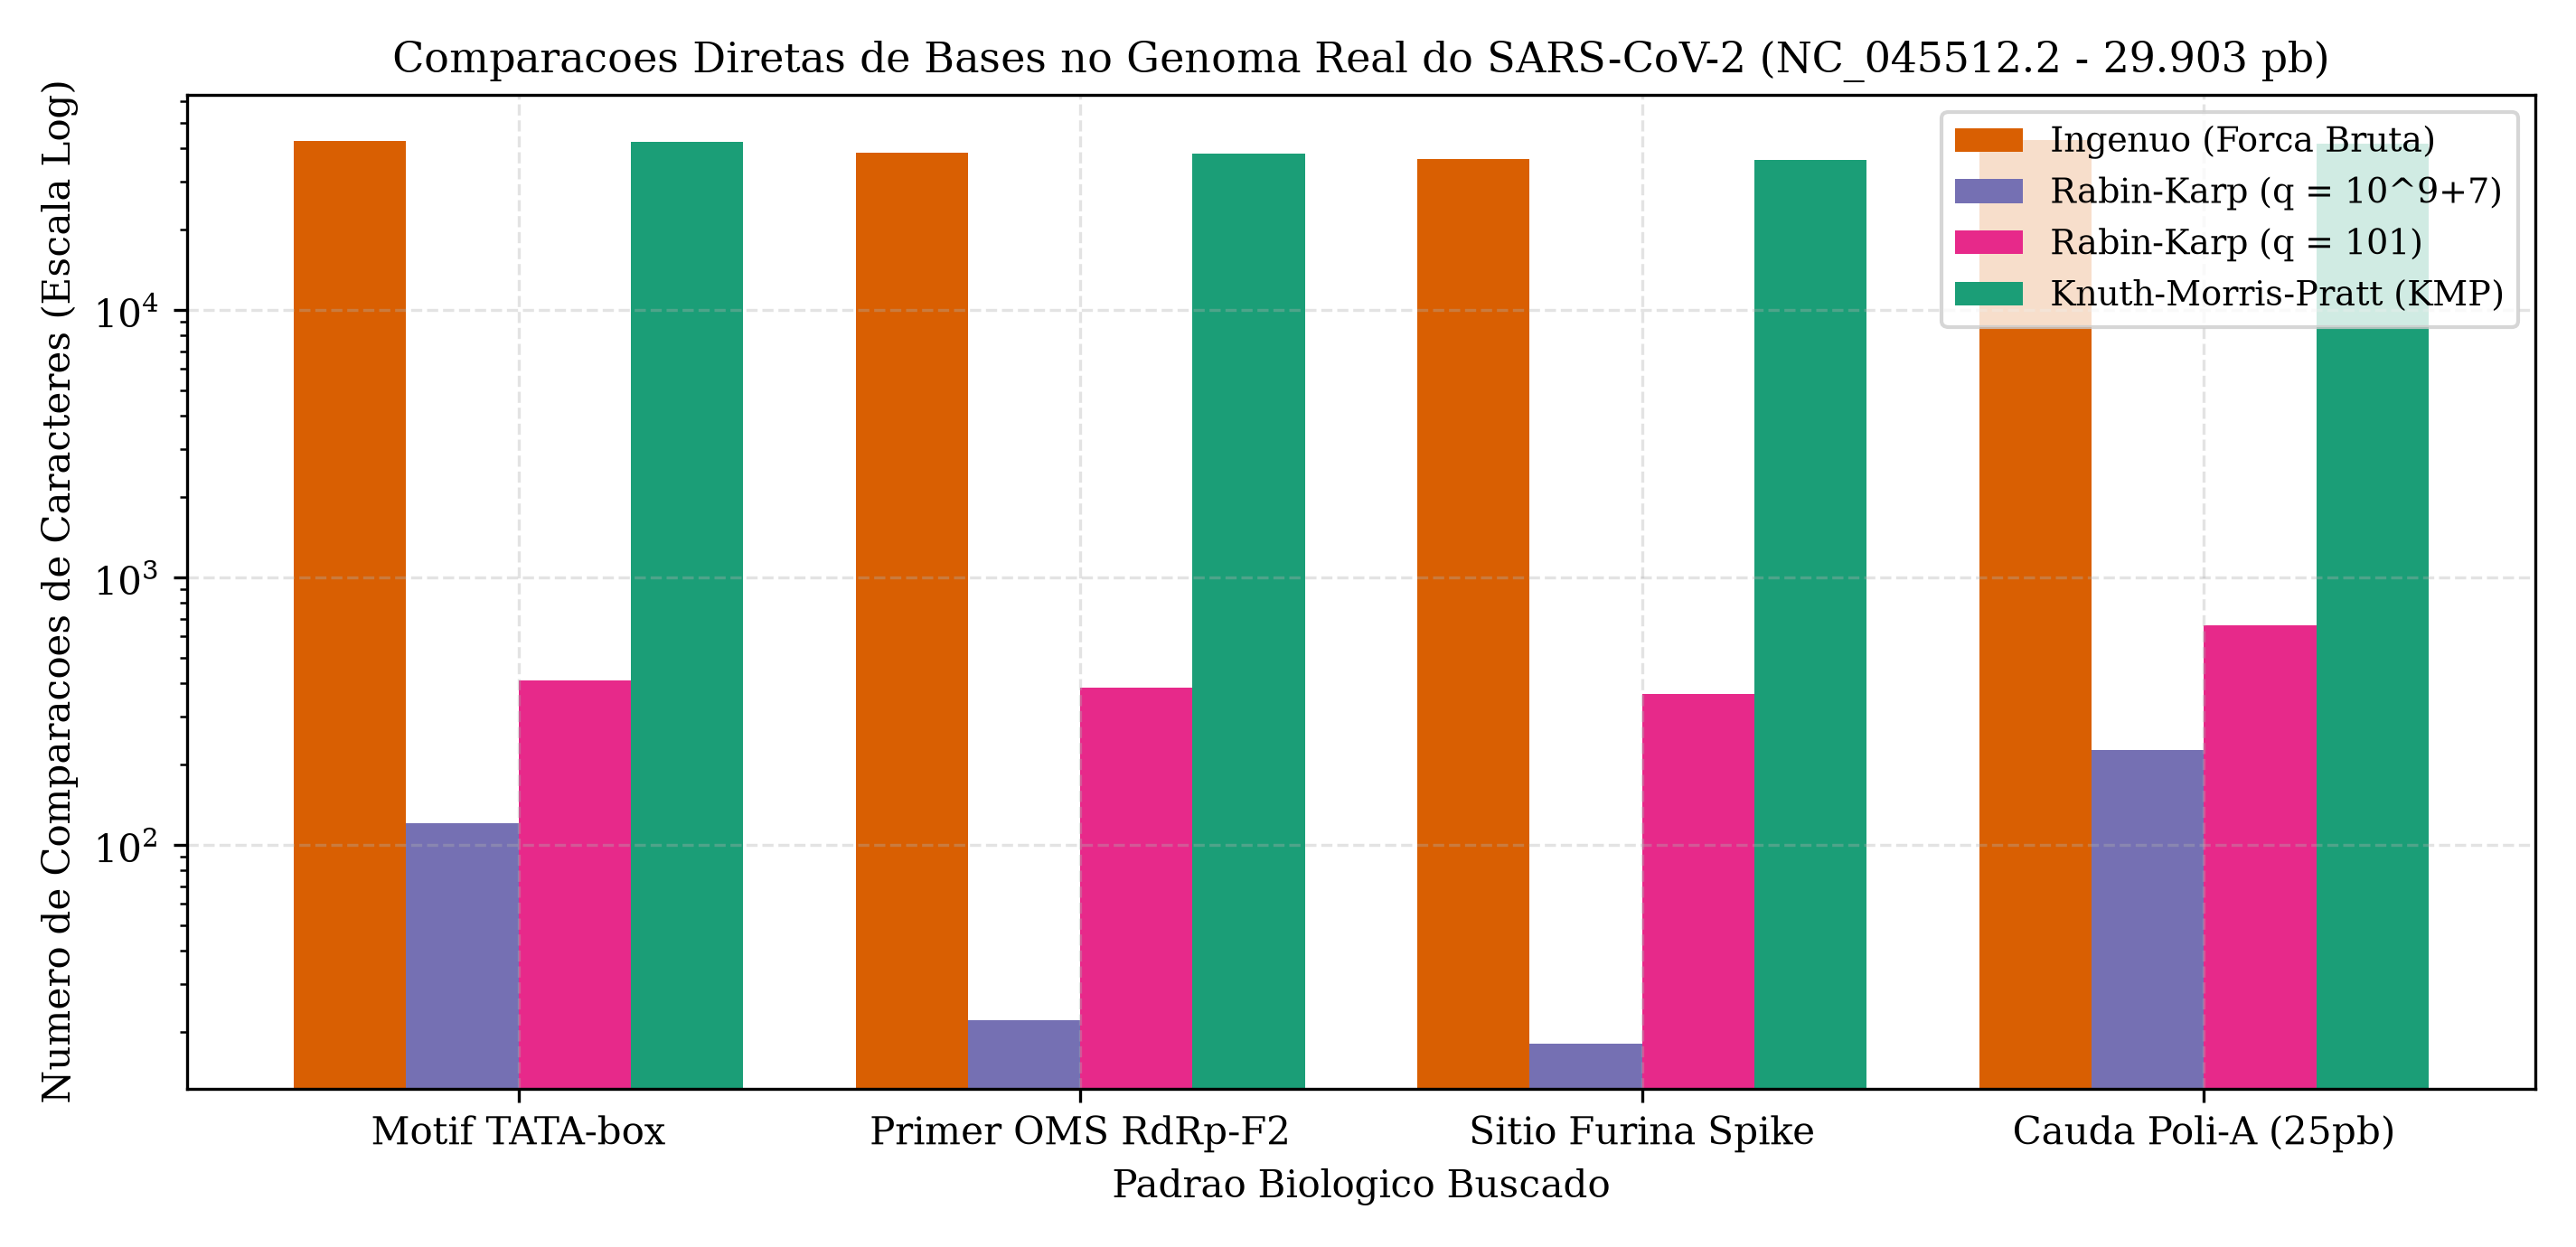
\includegraphics[width=0.88\textwidth]{comparacoes_genoma_sars.png}
    \caption{Compara\c{c}\~oes diretas de caracteres realizadas por cada algoritmo sobre o genoma do SARS-CoV-2.}
    \label{fig:genoma_sars}
\end{figure}

Adicionalmente, testamos na fun\c{c}\~ao \texttt{seeding\_rabin\_karp} a recupera\c{c}\~ao de uma leitura simulada de $120$ pb extra\'ida da posi\c{c}\~ao $21.562$ (in\'icio do gene \textit{Spike}) na qual introduzimos artificialmente duas muta\c{c}\~oes pontuais (SNPs) nos \'indices $35$ e $88$. Ao buscar a leitura inteira de $120$ pb com o KMP, o resultado foi de $0$ ocorr\^encias devido \`as duas bases divergentes. Em contrapartida, a etapa de \textit{seeding} via \textit{rolling hash} de Rabin-Karp ($k=15$) localizou instantaneamente $76$ \^ancoras exatas preservadas nos segmentos intactos da leitura, apontando exatamente para o deslocamento original $s = 21.562$ do genoma viral.

\subsection{Experimento 2: Escalabilidade Linear com Entradas Progressivas ($N$)}

Na Figura \ref{fig:escala_n}, avaliamos o comportamento com entradas progressivas de DNA pseudo-aleat\'orio variando de $N = 10.000$ pb at\'e $N = 5.000.000$ pb ($5$ Mpb), fixando $M = 64$ pb.

\begin{figure}[H]
    \centering
    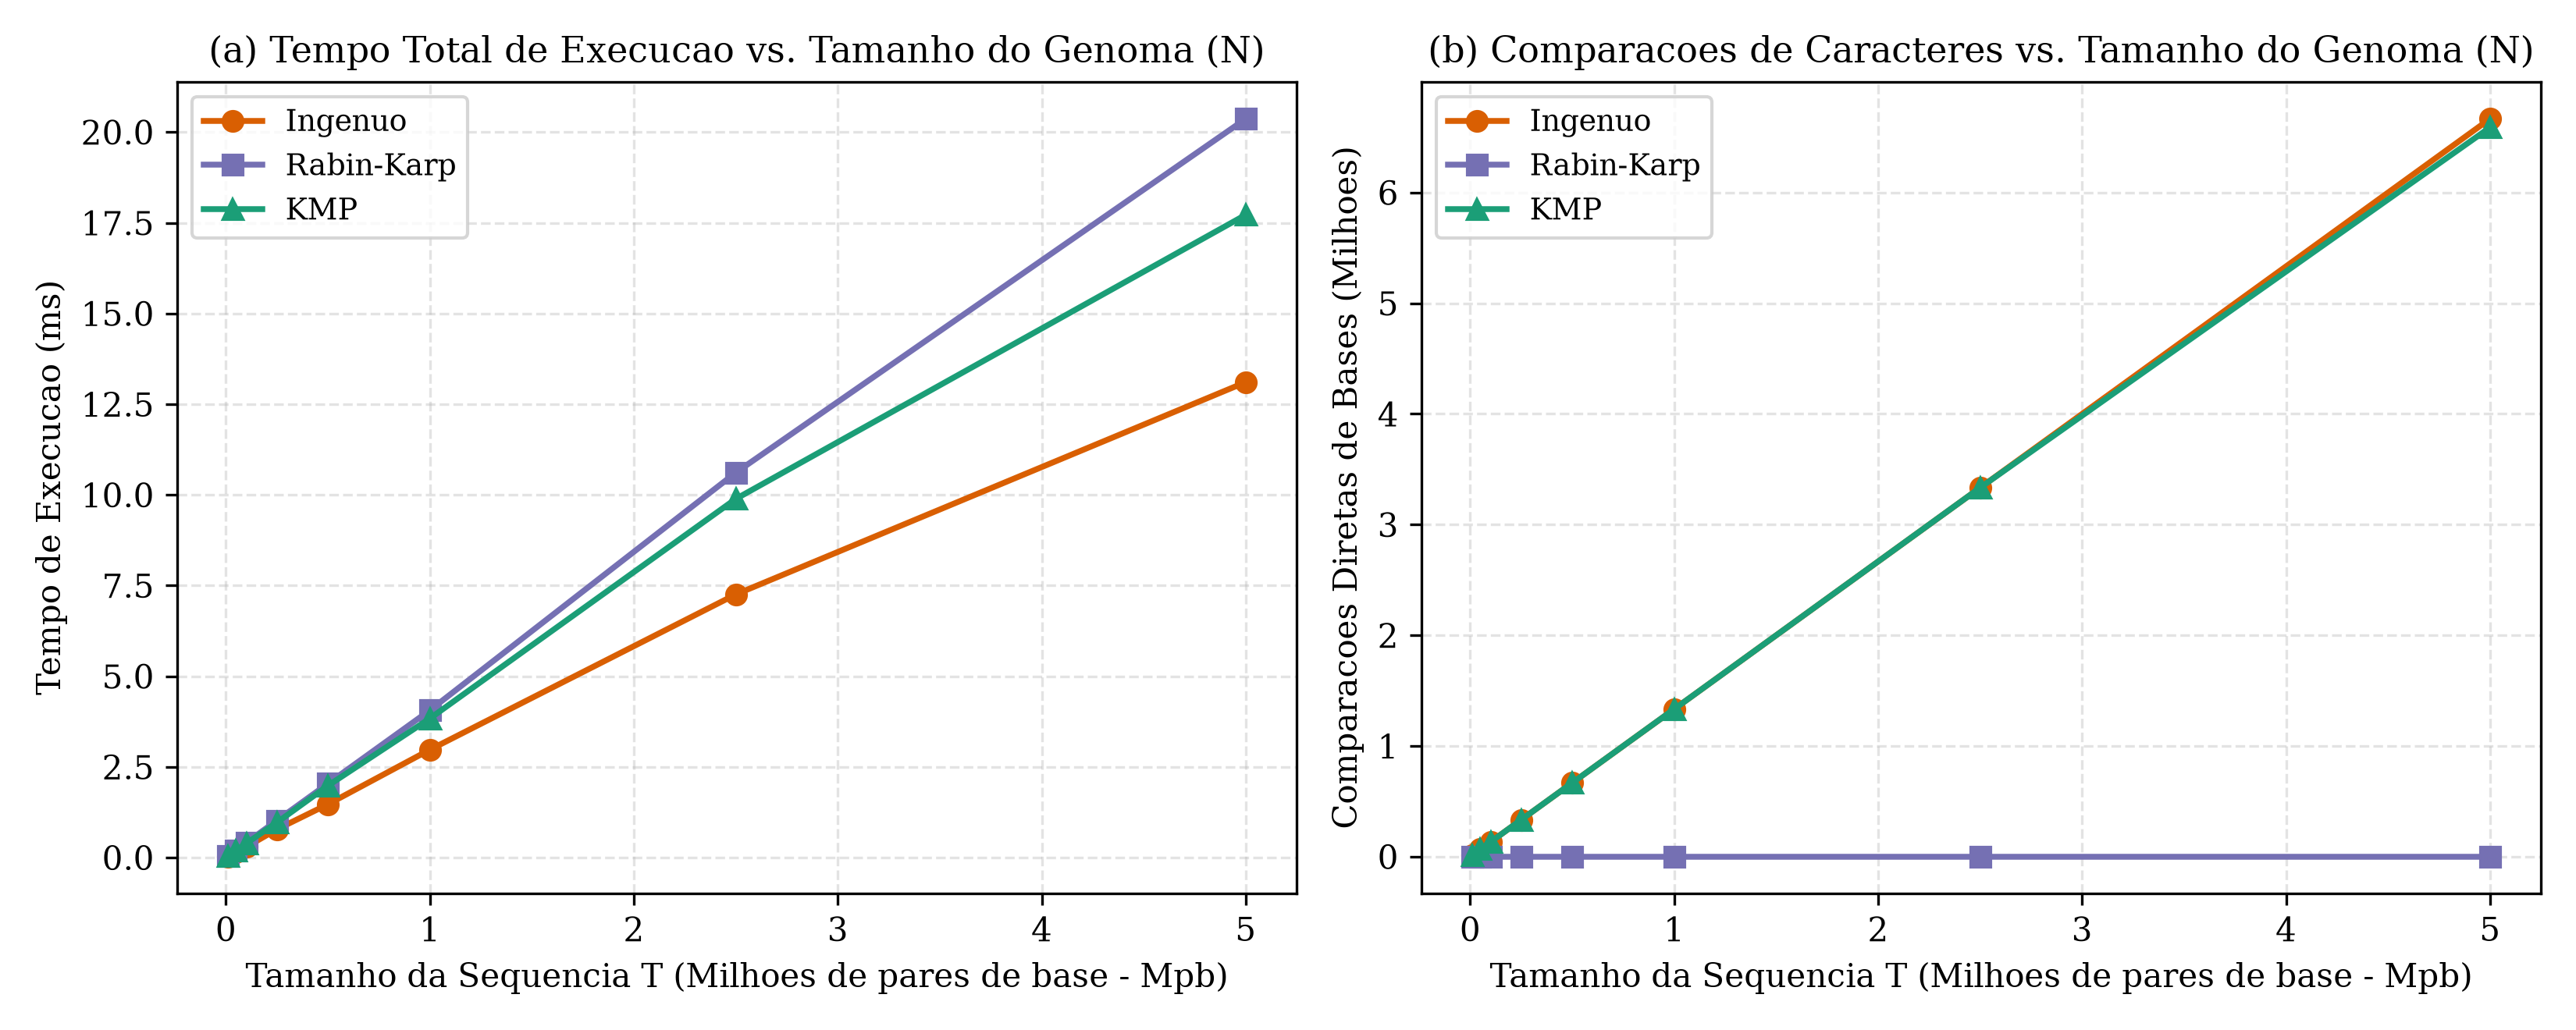
\includegraphics[width=0.98\textwidth]{tempo_escala_n.png}
    \caption{Evolu\c{c}\~ao do tempo de execu\c{c}\~ao (a) e do n\'umero de compara\c{c}\~oes (b) com entradas progressivas at\'e $5$ Mpb.}
    \label{fig:escala_n}
\end{figure}

Os dados confirmam visual e numericamente a linearidade $\Theta(n)$ dos tr\^es m\'etodos no caso m\'edio uniforme. Para $N = 5.000.000$ pb, tanto a busca ing\^enua quanto o KMP efetuam cerca de $6,66 \times 10^6$ compara\c{c}\~oes de caracteres ($\approx 1,33 \cdot N$, cravando a previs\~ao te\'orica de $\frac{4}{3}N$ deduzida na Se\c{c}\~ao 4.1).

\subsection{Experimento 3: Pior Caso Patol\'ogico em DNA Repetitivo e Impacto do Primo $q$}

Para expor a falha catastr\'ofica do algoritmo ing\^enuo em regi\~oes homopolim\'ericas de DNA, submetemos os algoritmos a uma sequ\^encia repetitiva poli-A de comprimento $N = 100.000$ pb com padr\~oes de tamanho $M \in \{50, 100, 250, 500, 1000, 2000\}$ da forma $\texttt{A}^{M-1}\texttt{C}$.

\begin{figure}[H]
    \centering
    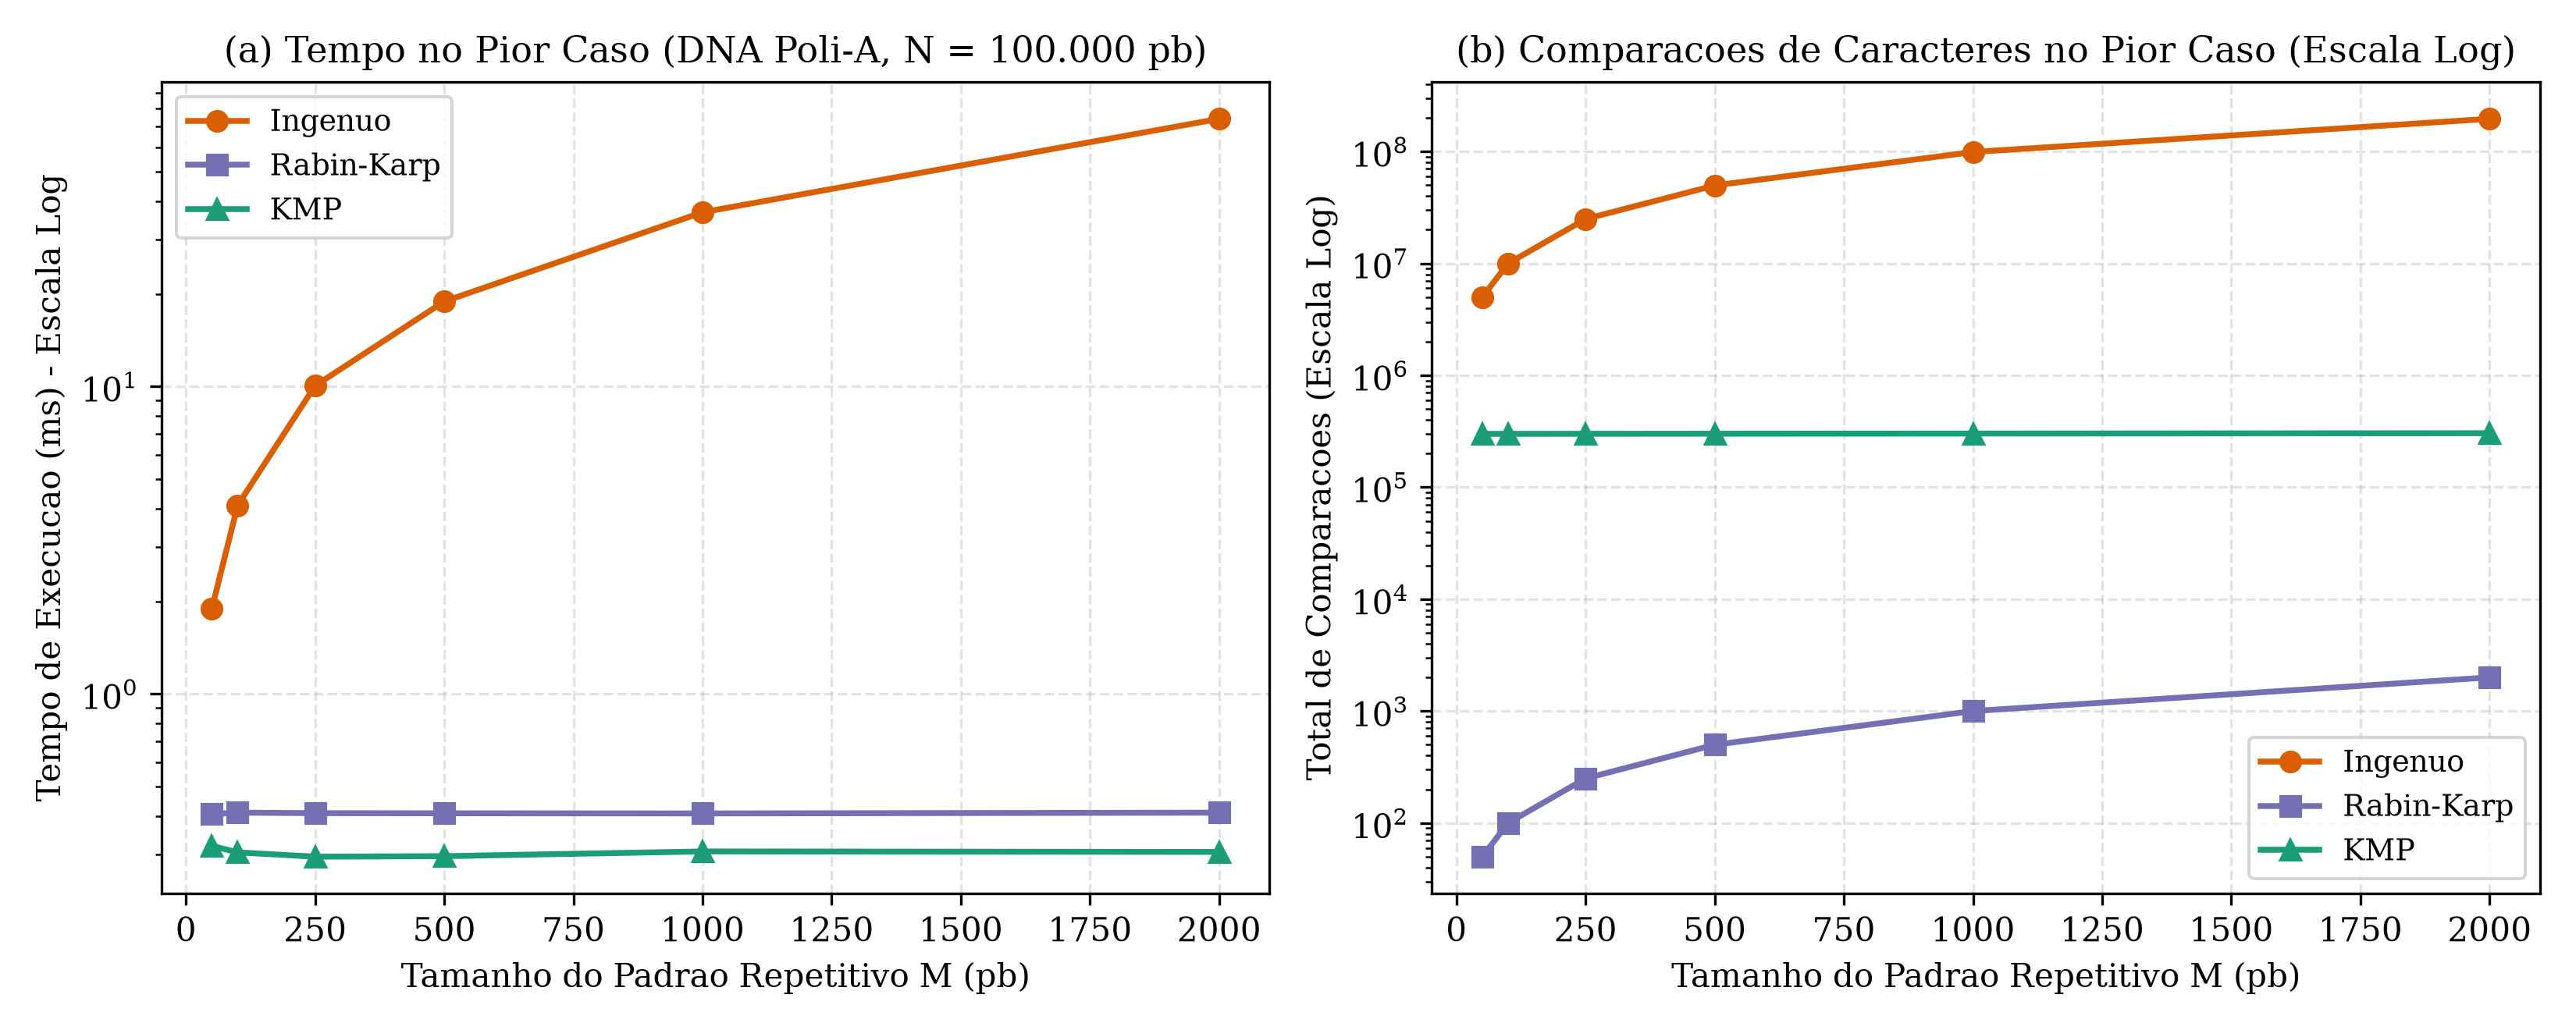
\includegraphics[width=0.98\textwidth]{pior_caso_repetitivo.png}
    \caption{Degrada\c{c}\~ao quadr\'atica $\Theta(nm)$ da busca ing\^enua versus estabilidade linear $\Theta(n+m)$ do KMP e Rabin-Karp em DNA repetitivo.}
    \label{fig:pior_caso}
\end{figure}

Os resultados na Figura \ref{fig:pior_caso} s\~ao contundentes: quando $M = 2.000$, a busca ing\^enua realiza exatas $196.002.000$ compara\c{c}\~oes e consome $74,17\text{ ms}$. O algoritmo KMP, consultando o vetor $\pi$, realiza apenas $303.993$ compara\c{c}\~oes e finaliza a busca em $0,306\text{ ms}$ (um ganho de velocidade de \textbf{242 vezes}), mantendo o tempo de busca inalterado ($\approx 0,30\text{ ms}$) independentemente do aumento de $M$.

Na Figura \ref{fig:colisoes_rk}, investigamos o impacto da escolha do m\'odulo primo $q$ sobre as colis\~oes esp\'urias no Rabin-Karp ($N = 500.000$ pb, $M = 32$ pb). Quando utilizamos um primo pequeno ($q = 13$), ocorrem $38.899$ falsos positivos de hash ($\approx N/13$), for\c{c}ando $51.802$ compara\c{c}\~oes extras de caracteres e elevando o tempo de busca para $2,53\text{ ms}$. Ao escalar o primo para $q = 10^9 + 7$, o n\'umero de colis\~oes esp\'urias cai para zero absoluto, restringindo as compara\c{c}\~oes de caracteres \`as $32$ bases da \'unica ocorr\^encia real.

\begin{figure}[H]
    \centering
    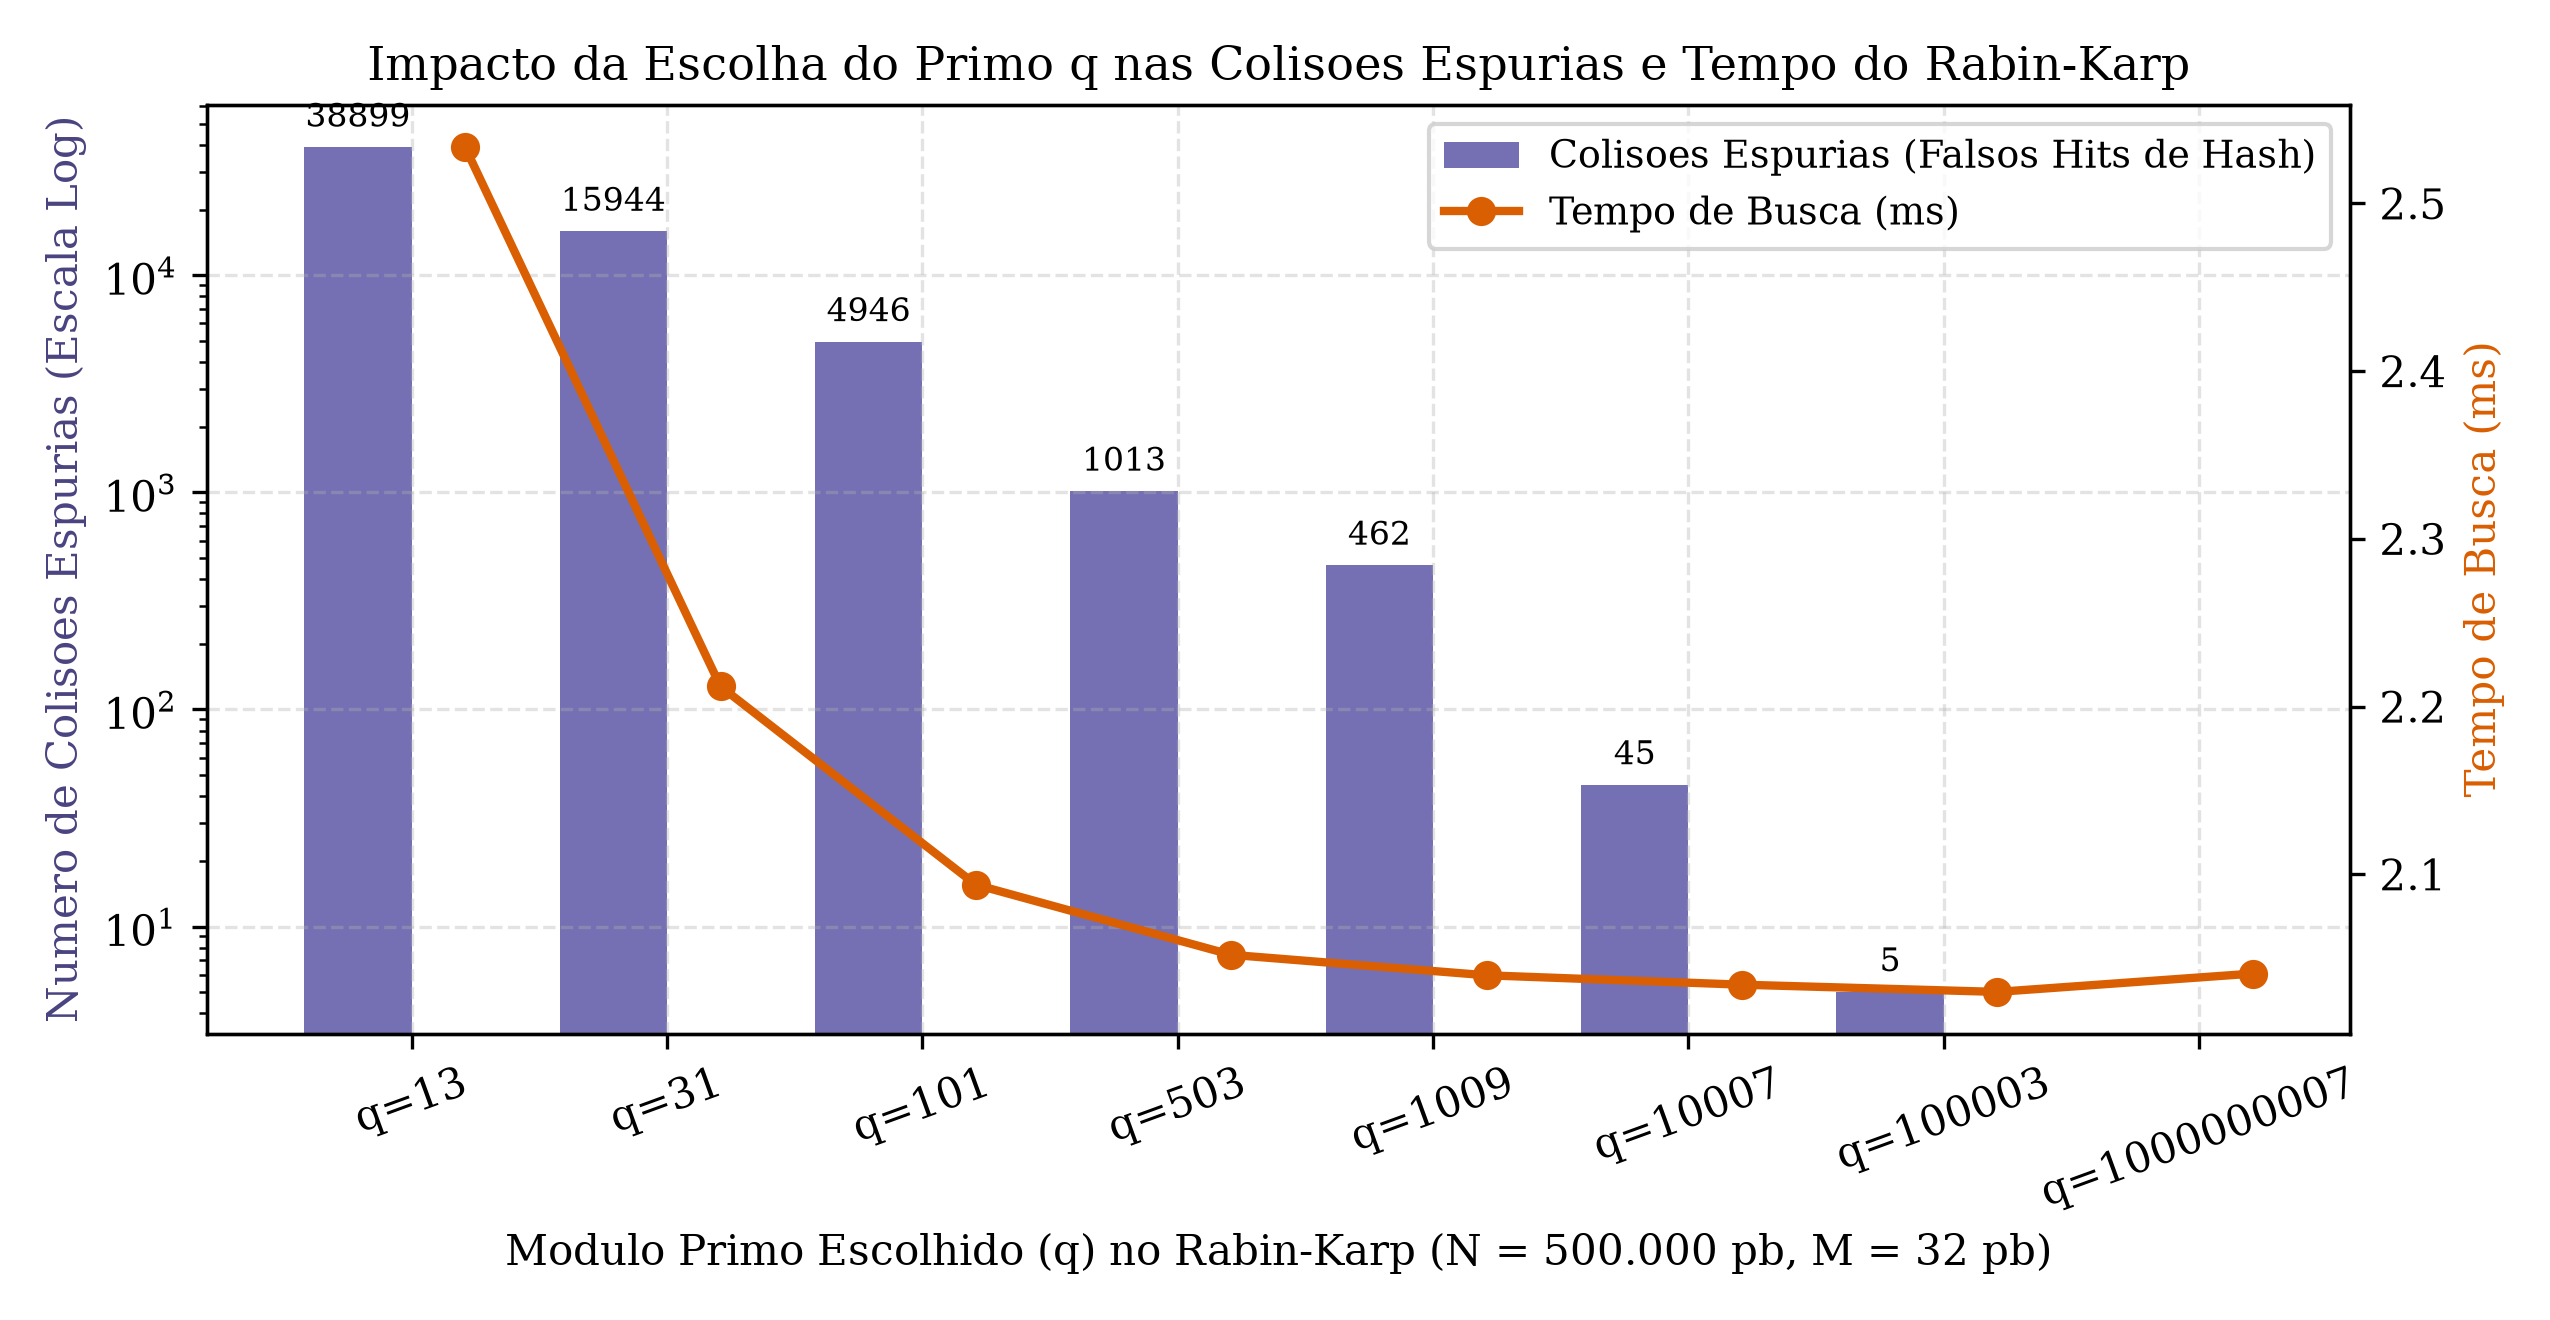
\includegraphics[width=0.84\textwidth]{colisoes_rabin_karp.png}
    \caption{Decaimento logar\'itmico das colis\~oes esp\'urias e redu\c{c}\~ao do tempo de busca no Rabin-Karp em fun\c{c}\~ao do primo $q$.}
    \label{fig:colisoes_rk}
\end{figure}

\subsection{Discuss\~ao Cr\'itica: Gargalos de Hardware e de Linguagem em C++17}

A an\'alise conjunta dos resultados pr\'aticos revela nuances de arquitetura de computadores que a nota\c{c}\~ao assint\'otica pura omite:
\begin{enumerate}
    \item \textbf{Lat\^encia da Instru\c{c}\~ao de Divis\~ao/M\'odulo na ALU (\texttt{idiv}):} Na Figura \ref{fig:escala_n}(a), observa-se que, em DNA uniforme aleat\'orio ($N = 5$ Mpb), o Rabin-Karp levou $20,36\text{ ms}$ frente a $17,71\text{ ms}$ do KMP e $13,10\text{ ms}$ do algoritmo ing\^enuo, mesmo tendo efetuado apenas $64$ compara\c{c}\~oes diretas de caracteres! Isso ocorre porque, para cada um dos $5$ milh\~oes de deslocamentos, o Rabin-Karp executa a opera\c{c}\~ao \texttt{\% q} sobre inteiros de 64 bits. Em arquiteturas x86\_64, o operador \texttt{\%} com divisor vari\'avel compila para a instru\c{c}\~ao \texttt{idiv}, cuja lat\^encia na unidade l\'ogico-aritm\'etica (ALU) varia de $20$ a $40$ ciclos de clock, enquanto a instru\c{c}\~ao \texttt{cmp} de 1 byte na mem\'oria cache L1 executada pela busca ing\^enua consome apenas $1$ ciclo de clock.
    \item \textbf{Sem\^antica do Operador \texttt{\%} para Dividendos Negativos em C/C++:} Diferentemente da defini\c{c}\~ao matem\'atica de $\bmod q$ adotada no Cormen (que sempre retorna valores em $[0, q-1]$), o padr\~ao ISO C++ define \texttt{a \% b} com o mesmo sinal do dividendo \texttt{a}. Na subtra\c{c}\~ao do d\'igito mais significativo \texttt{t - char\_sai * h}, o resultado frequentemente se torna negativo, o que corromperia todos os hashes subsequentes caso n\~ao inclu\'issemos a corre\c{c}\~ao expl\'icita:
\begin{lstlisting}[language=C++, caption=Tratamento de overflow e resto negativo no Rolling Hash em C++17]
int64_t char_sai = static_cast<unsigned char>(T[s]);
int64_t char_entra = static_cast<unsigned char>(T[s + m]);
t = (d * (t - char_sai * h) + char_entra) % q;
if (t < 0) {
    t += q; // Ajusta o resto truncado do C++ para o representante positivo em Z_q
}
\end{lstlisting}
    \item \textbf{Preven\c{c}\~ao de \textit{Integer Overflow} e Convers\~ao de \'Indices Base-0:} Caso utiliz\'assemos o tipo padr\~ao \texttt{int} (32 bits, limite $2,14 \times 10^9$) com $q = 10^9 + 7$ e $d = 256$, o produto intermedi\'ario $d \cdot (t - \text{char\_sai} \cdot h)$ alcan\c{c}aria a ordem de $2,56 \times 10^{11}$, provocando \textit{signed integer overflow} (comportamento indefinido em C++). O uso estrito de \texttt{int64\_t} (limite $9,22 \times 10^{18}$) elimina esse gargalo. No KMP, a adapta\c{c}\~ao da nota\c{c}\~ao base-1 do Cormen (\texttt{k = pi[k]}) para vetores base-0 em C++ exigiu mapear o recuo de estado para \texttt{k = pi[k - 1]}, mantendo o vetor $\pi$ cont\'iguo na cache L1 ($256$ bytes para $M=64$).
\end{enumerate}

% =============================================================================
% 6. CONCLUSOES E REFERENCIAS BIBLIOGRAFICAS
% =============================================================================
\section{Conclus\~oes}

O estudo te\'orico e experimental desenvolvido neste trabalho permitiu confrontar a eleg\^ancia matem\'atica dos algoritmos de casamento de cadeias com a realidade f\'isica de sua execu\c{c}\~ao sobre dados gen\^omicos. Ficou demonstrado que cada abordagem possui um nicho de superioridade bem delimitado:

\begin{itemize}
    \item \textbf{Onde o KMP \'e imbat\'ivel:} Na busca determin\'istica de um \'unico padr\~ao sobre alfabetos pequenos ($|\Sigma|=4$ no DNA) ou textos sujeitos a repeti\c{c}\~oes peri\'odicas (caudas poli-A, repeti\c{c}\~oes em tandem). O KMP oferece garantia estrita de tempo $\Theta(n+m)$ no pior caso, sem depender de escolhas de n\'umeros primos e realizando apenas compara\c{c}\~oes leves na cache L1.
    \item \textbf{Onde o Rabin-Karp se destaca:} Na busca simult\^anea de \textbf{m\'ultiplos padr\~oes} de comprimento fixo (como na indexa\c{c}\~ao de dezenas de milhares de $k$-mers em uma tabela hash durante a etapa de \textit{seeding} de alinhadores gen\'eticos) e no casamento de padr\~oes bidimensionais. Enquanto o KMP exigiria construir um aut\^omato de Aho-Corasick com alto consumo de mem\'oria para múltiplos padrões, o Rabin-Karp calcula o hash da janela do texto uma \'unica vez em $\Theta(1)$ e consulta o dicion\'ario de sementes instantaneamente.
    \item \textbf{Onde o paradigma falha:} Tanto o KMP quanto o Rabin-Karp puro falham quando o problema exige toler\^ancia direta a muta\c{c}\~oes pontuais (SNPs) ou inser\c{c}\~oes/dele\c{c}\~oes (\textit{indels}) ao longo de toda a cadeia sem subdivis\~ao em sementes. Nesses cen\'arios aproximados, ou quando o mesmo genoma est\'atico de refer\^encia ser\'a consultado milh\~oes de vezes, o paradigma de varredura on-line $\Theta(n)$ cede espa\c{c}o para estruturas de indexa\c{c}\~ao pr\'evia do texto (como Suffix Arrays e a Transformada de Burrows-Wheeler com FM-Index \cite{li2009}, que reduzem a busca para $O(m)$) combinadas com programa\c{c}\~ao din\^amica local.
\end{itemize}

\begin{thebibliography}{9}

\bibitem{cormen2022}
CORMEN, T. H.; LEISERSON, C. E.; RIVEST, R. L.; STEIN, C. \textbf{Algoritmos: Teoria e Pr\'atica}. 3. ed. Rio de Janeiro: Elsevier / GEN LTC, 2012. Cap. 32 (Casamento de Cadeias), p. 719--745.

\bibitem{knuth1977}
KNUTH, D. E.; MORRIS, J. H.; PRATT, V. R. Fast pattern matching in strings. \textbf{SIAM Journal on Computing}, v. 6, n. 2, p. 323--350, 1977. DOI: \url{https://doi.org/10.1137/0206024}.

\bibitem{karp1987}
KARP, R. M.; RABIN, M. O. Efficient randomized pattern-matching algorithms. \textbf{IBM Journal of Research and Development}, v. 31, n. 2, p. 249--260, 1987. DOI: \url{https://doi.org/10.1147/rd.312.0249}.

\bibitem{altschul1990}
ALTSCHUL, S. F.; GISH, W.; MILLER, W.; MYERS, E. W.; LIPMAN, D. J. Basic local alignment search tool. \textbf{Journal of Molecular Biology}, v. 215, n. 3, p. 403--410, 1990. DOI: \url{https://doi.org/10.1006/jmbi.1990.9999}.

\bibitem{li2009}
LI, H.; DURBIN, R. Fast and accurate short read alignment with Burrows-Wheeler transform. \textbf{Bioinformatics}, v. 25, n. 14, p. 1754--1760, 2009. DOI: \url{https://doi.org/10.1093/bioinformatics/btp324}.


\bibitem{repo2026}
MENDON\c{C}A, A. O.; FONSECA, I. X.; MARTINS, T. A. S.; GUERREIRO, T.; TAVARES, M. \textbf{Implementa\c{c}\~ao e An\'alise Experimental de Algoritmos de Casamento de Cadeias (Rabin-Karp e KMP) em Sequ\^encias Gen\^omicas}. Reposit\'orio p\'ublico de c\'odigo-fonte e experimentos no GitHub, 2026. Dispon\'ivel em: \url{https://github.com/ImArthz/Aeds2_casamento_de_cadeias.git}. Acesso em: 02 nov. 2026.

\end{thebibliography}

\newpage

% =============================================================================
% APENDICE EXIGIDO: CHEAT SHEET (GUIA DE CONSULTA RAPIDA - 1 PAGINA)
% =============================================================================
\appendix\setstretch{1.12}
\section*{Ap\^endice: Cheat Sheet -- Casamento de Cadeias (Cap. 32)}
\addcontentsline{toc}{section}{Ap\^endice: Cheat Sheet (Guia de Consulta R\'apida)}

\vspace{-0.2cm}
\noindent\fcolorbox{black!70}{blue!6}{%
\parbox{0.97\textwidth}{%
\textbf{a) Defini\c{c}\~ao do Paradigma em Uma Frase:} \\
Localizar todas as posi\c{c}\~oes de ocorr\^encia de um padr\~ao $P[1..m]$ dentro de um texto $T[1..n]$ em tempo linear $\Theta(n+m)$, substituindo re-compara\c{c}\~oes redundantes por impress\~oes digitais aritm\'eticas (\textit{Rolling Hash} no Rabin-Karp) ou transi\c{c}\~oes de estado baseadas em auto-sobreposi\c{c}\~ao de prefixos (Tabela $\pi$ no KMP).
}}

\vspace{0.25cm}
\noindent\textbf{b) Diagrama de Decis\~ao: ``Quando Utilizar Esta Abordagem?''}

\begin{center}
\begin{tikzpicture}[
    node distance=0.45cm and 0.9cm,
    qbox/.style={rectangle, rounded corners, draw=black!80, fill=orange!12, text width=3.6cm, align=center, inner sep=4pt, font=\scriptsize\bfseries},
    ans/.style={rectangle, draw=black!80, fill=green!12, text width=3.5cm, align=center, inner sep=4pt, font=\scriptsize},
    arr/.style={-{Stealth[length=2mm]}, thick}
]
    \node[qbox] (q1) {Precisa tolerar muta\c{c}\~oes/gaps na cadeia inteira?};
    \node[ans, right=1.2cm of q1] (a1) {\textbf{Seeding (Rabin-Karp $k$-mers)} + \textbf{Prog. Din\^amica} (Smith-Waterman)};
    \node[qbox, below=of q1] (q2) {Busca m\'ultiplos padr\~oes simult\^aneos ou 2D?};
    \node[ans, right=1.2cm of q2] (a2) {\textbf{Rabin-Karp} (\textit{Rolling Hash} em Tabela Hash: $\Theta(n + km)$ m\'edio)};
    \node[qbox, below=of q2] (q3) {Alfabeto pequeno (DNA) ou exig\^encia de pior caso linear?};
    \node[ans, right=1.2cm of q3] (a3) {\textbf{Knuth-Morris-Pratt (KMP)} (Garantia determin\'istica $\Theta(n+m)$)};
    \node[ans, below=0.55cm of q3, fill=gray!15] (a4) {\textbf{Busca Ing\^enua} ($m$ muito curto, texto pequeno e mem\'oria $\Theta(1)$)};

    \draw[arr] (q1) -- node[above, font=\tiny\bfseries] {SIM} (a1);
    \draw[arr] (q1) -- node[left, font=\tiny\bfseries] {N\~AO (Exato)} (q2);
    \draw[arr] (q2) -- node[above, font=\tiny\bfseries] {SIM} (a2);
    \draw[arr] (q2) -- node[left, font=\tiny\bfseries] {N\~AO (1 Padr\~ao)} (q3);
    \draw[arr] (q3) -- node[above, font=\tiny\bfseries] {SIM} (a3);
    \draw[arr] (q3) -- node[left, font=\tiny\bfseries] {N\~AO} (a4);
\end{tikzpicture}
\end{center}

\vspace{-0.15cm}
\noindent\textbf{c) Tabela Resumo das Complexidades de Tempo e Espa\c{c}o}

\begin{table}[H]
\centering
\scriptsize
\resizebox{\textwidth}{!}{\begin{tabular}{@{}lccccc@{}}
\toprule
\textbf{Algoritmo} & \textbf{Pr\'e-processamento} & \textbf{Melhor Caso ($\Omega$)} & \textbf{Caso M\'edio ($\Theta$)} & \textbf{Pior Caso ($O / \Theta$)} & \textbf{Espa\c{c}o Auxiliar} \\ \midrule
\textbf{Ing\^enuo (For\c{c}a Bruta)} & $0$ (Nenhum) & $\Omega(n)$ & $\Theta(n)$ & $\Theta((n-m+1)m)$ & $\Theta(1)$ \\
\textbf{Rabin-Karp} & $\Theta(m)$ & $\Omega(n - m + 1)$ & $\Theta(n + m)$ & $\Theta((n-m+1)m)$ & $\Theta(1)$ \\
\textbf{Knuth-Morris-Pratt (KMP)} & $\Theta(m)$ & $\Omega(n + m)$ & $\Theta(n + m)$ & $\Theta(n + m)$ & $\Theta(m)$ \\ \bottomrule
\end{tabular}}
\end{table}

\vspace{-0.2cm}
\noindent\textbf{d) Esqueleto Base da T\'ecnica (Rabin-Karp \& KMP em Base-0)}

\begin{lstlisting}[language=C++, basicstyle=\ttfamily\scriptsize, numbers=none]
// 1. ESQUELETO KMP: Construcao de pi em Theta(m) + Busca sem retrocesso em Theta(n)
vector<int> pi(m, 0);
for (int q = 1, k = 0; q < m; ++q) {
    while (k > 0 && P[k] != P[q]) k = pi[k - 1]; // Recua pelo maior sufixo-prefixo
    if (P[k] == P[q]) k++;
    pi[q] = k;
}
for (int i = 0, q = 0; i < n; ++i) {
    while (q > 0 && P[q] != T[i]) q = pi[q - 1]; // i nunca retrocede!
    if (P[q] == T[i]) q++;
    if (q == m) { reportar_match(i + 1 - m); q = pi[q - 1]; }
}

// 2. ESQUELETO RABIN-KARP: Atualizacao O(1) do Rolling Hash via Aritmetica Modular
// Pre-calculo: h = d^(m-1) mod q; p e t calculados via Regra de Horner nos primeiros m chars
for (int s = 0; s <= n - m; ++s) {
    if (p == t && T.compare(s, m, P) == 0) reportar_match(s); // Filtra colisao espuria
    if (s < n - m) {
        t = (d * (t - T[s] * h) + T[s + m]) % q;
        if (t < 0) t += q; // Garante residuo positivo em Z_q
    }
}
\end{lstlisting}

\end{document}
